\documentclass[12pt,a4paper]{article}
\usepackage[latin1]{inputenc}
\usepackage{amsmath}
\usepackage{amsfonts}
\usepackage{amssymb}
\usepackage{graphicx}
\graphicspath{ {./images/} }
\usepackage{mwe}
\usepackage{wrapfig}
\usepackage{enumitem}
\usepackage[hidelinks]{hyperref}
\hypersetup{urlcolor=blue, colorlinks=true, linkcolor=black}
\author{Zdenek Krousky}
\title{Easysleep}
\hyphenation{con-sti-tu-tion-al}
\usepackage{listings}
\usepackage{color}

\definecolor{dkgreen}{rgb}{0,0.6,0}
\definecolor{gray}{rgb}{0.5,0.5,0.5}
\definecolor{mauve}{rgb}{0.58,0,0.82}
\definecolor{light_gray}{rgb}{0.9, 0.9, 0.9}

\lstset{frame=tb,
  language=C++,
  aboveskip=3mm,
  belowskip=3mm,
  showstringspaces=false,
  columns=flexible,
  basicstyle={\small\ttfamily},
  numbers=none,
  backgroundcolor=\color{light_gray},
  numberstyle=\tiny\color{gray},
  keywordstyle=\color{blue},
  commentstyle=\color{dkgreen},
  stringstyle=\color{mauve},
  breaklines=true,
  breakatwhitespace=true,
  tabsize=3
}

\renewcommand*\contentsname{Table of Content}
\renewcommand{\lstlistlistingname}{Code listings}

\begin{document}
	\begin{titlepage}
		\centering
		
\includegraphics[width=0.5\textwidth]{gmit_full1.png}\par\vspace{0cm}
		{\scshape\LARGE Galway - Mayo \par Institute of Technology \par}
		\vspace{1cm}
		{\scshape\Large Final year project\par}
		\vspace{1.5cm}
		{\Huge\bfseries Easysleep\par}
		\vspace{2cm}
		{\Large\itshape Zdenek Krousky\par}
		\vfill
		supervised by\par
		Paul \textsc{Lennon}
		
		\vfill
		
		% Bottom of the page
		{\large \today\par}
	\end{titlepage}
	
	\newpage
	\pagenumbering{gobble}
	\pagenumbering{arabic}
	\newpage
	
	\section*{Declaration}
	This project is presented in partial fulfilment of the requirements for the Degree of Bachelor of Engineering (Hons.) in Software and Electronic Engineering at Galway-Mayo Institute of Technology. This project is my own work, except where otherwise accredited. Where the work of others has been used or incorporated during this project, this is acknowledged and referenced.
	\newpage
	
	\section*{Acknowledgement}
	I would like to extend my thanks to my supervisor Paul Lennon who made sure I stayed on track with my project, Niall O'Keeffe for his support in embedded part of the project, Michael Murray for his advice on the Android application development and to Michael Keaveney for going the extra mile to support me on the hardware side of things during the pandemic crisis. I would also like to thank my wife Caroline for her ongoing support through my studies.
	\newpage
	\tableofcontents
	\newpage
	
	\section{Project background and motivation}
	{\bfseries Aim of the project, Why?}\\
	The aim of this project was to create a device that would help to resolve nocturnal enurism, also known as bedwetting, which is common in children above the age of 5. I am the parent of a child with this issue and can relate to the stress this can cause to the child and the parents/guardians. My wife and I have tried various methods of resolving this - such as encouriging our daughter to go the toilet prior to going to the bed, restricting fluid intake before bed-time and waking her up during the night, yet none of these worked for us.\\
	
	According to my research there are a number of different causes for bedwetting and medical reasons account only for 3\% of these. 15\% of children above the age of 5 still wet the bed at night and up to 5\% above the age of 10 continue to do so. The selection of ``night-time training pants'' available in supermarkets go up to the age of 14, indicating that this issue can persist into the early teenage years in some cases.\\
	
	Having observed my daughter for several years, I have come to the conclusion that the main cause of her betwetting is deep sleep, i.e. her urge to go to the toilet simply isn't strong enough to wake her up at night. In addition, she is also very sensitive to loud noises and therefore my wife and I felt that introducing a bed-wetting alarm sheet might cause her unneccessary anxiety.\\
	
	This is where my project comes in - it aims to resolve nocturnal enurism in children 
	where deep sleep is the root cause in a somewhat gentler and smarter way than a bed-wetting
	alarm. 
	\newpage
	
	\section{Overview}
	{\bfseries What is Easysleep?, Research, Architecture diagram}\\
	
	The project consists of two devices that are able to communicate via Bluetooth and a mobile phone application. These are 2 FRDM-K64F microcontrollers. One assumes the role of a master and 
	monitors the moisture detection sensor, records the time and date of the event, sends a
	notification to the secondary device to wake the sleeping person up and if requested, 
	transfers time and date of last 10 events to the mobile phone application. It also notifies the 
	parent/guardian's phone if an event happens and activates the buzzer on the sleeping 
	person's bracelet.\\
	
	The secondary device (slave) uses a Parallax vibration motor to wake the sleeping person up. 
	If this is not acknowledged by pushing a button (indicating that he/she is awake) a second stage is entered and a buzzer is sounded.\\
	
	The mobile phone application allows the user to silence an ongoing alarm remotely, request 
	event data from the master device and save those into an SQLite database and check/change the 
	system time and date.\\
	\newpage
	
	\section{Hardware}
	{\bfseries Hardware used, Connections, Specifications}\\
	
	My project consists of the following hardware:
	
	\begin{itemize}
	 \item 2x FRDM-K64F development board used as the brains of the Easysleep master device and Easysleep bracelet device
	 \item 3x HC-05 Bluetooth module used for communication between master and slave devices as well as between the master and the mobile phone
	 \item Parallax vibration motor with interfacing circuit used in first stage to wake the sleeping person up by vibrations
	 \item Buzzer used in third stage as the final, most disruptive method of waking the sleeping  person up
	 \item Relay used in second stage, to bring a light up in the room of the sleeping person
	\end{itemize}

		\subsection{FRDM-K64F}
		\begin{figure}[h]
			\centering
			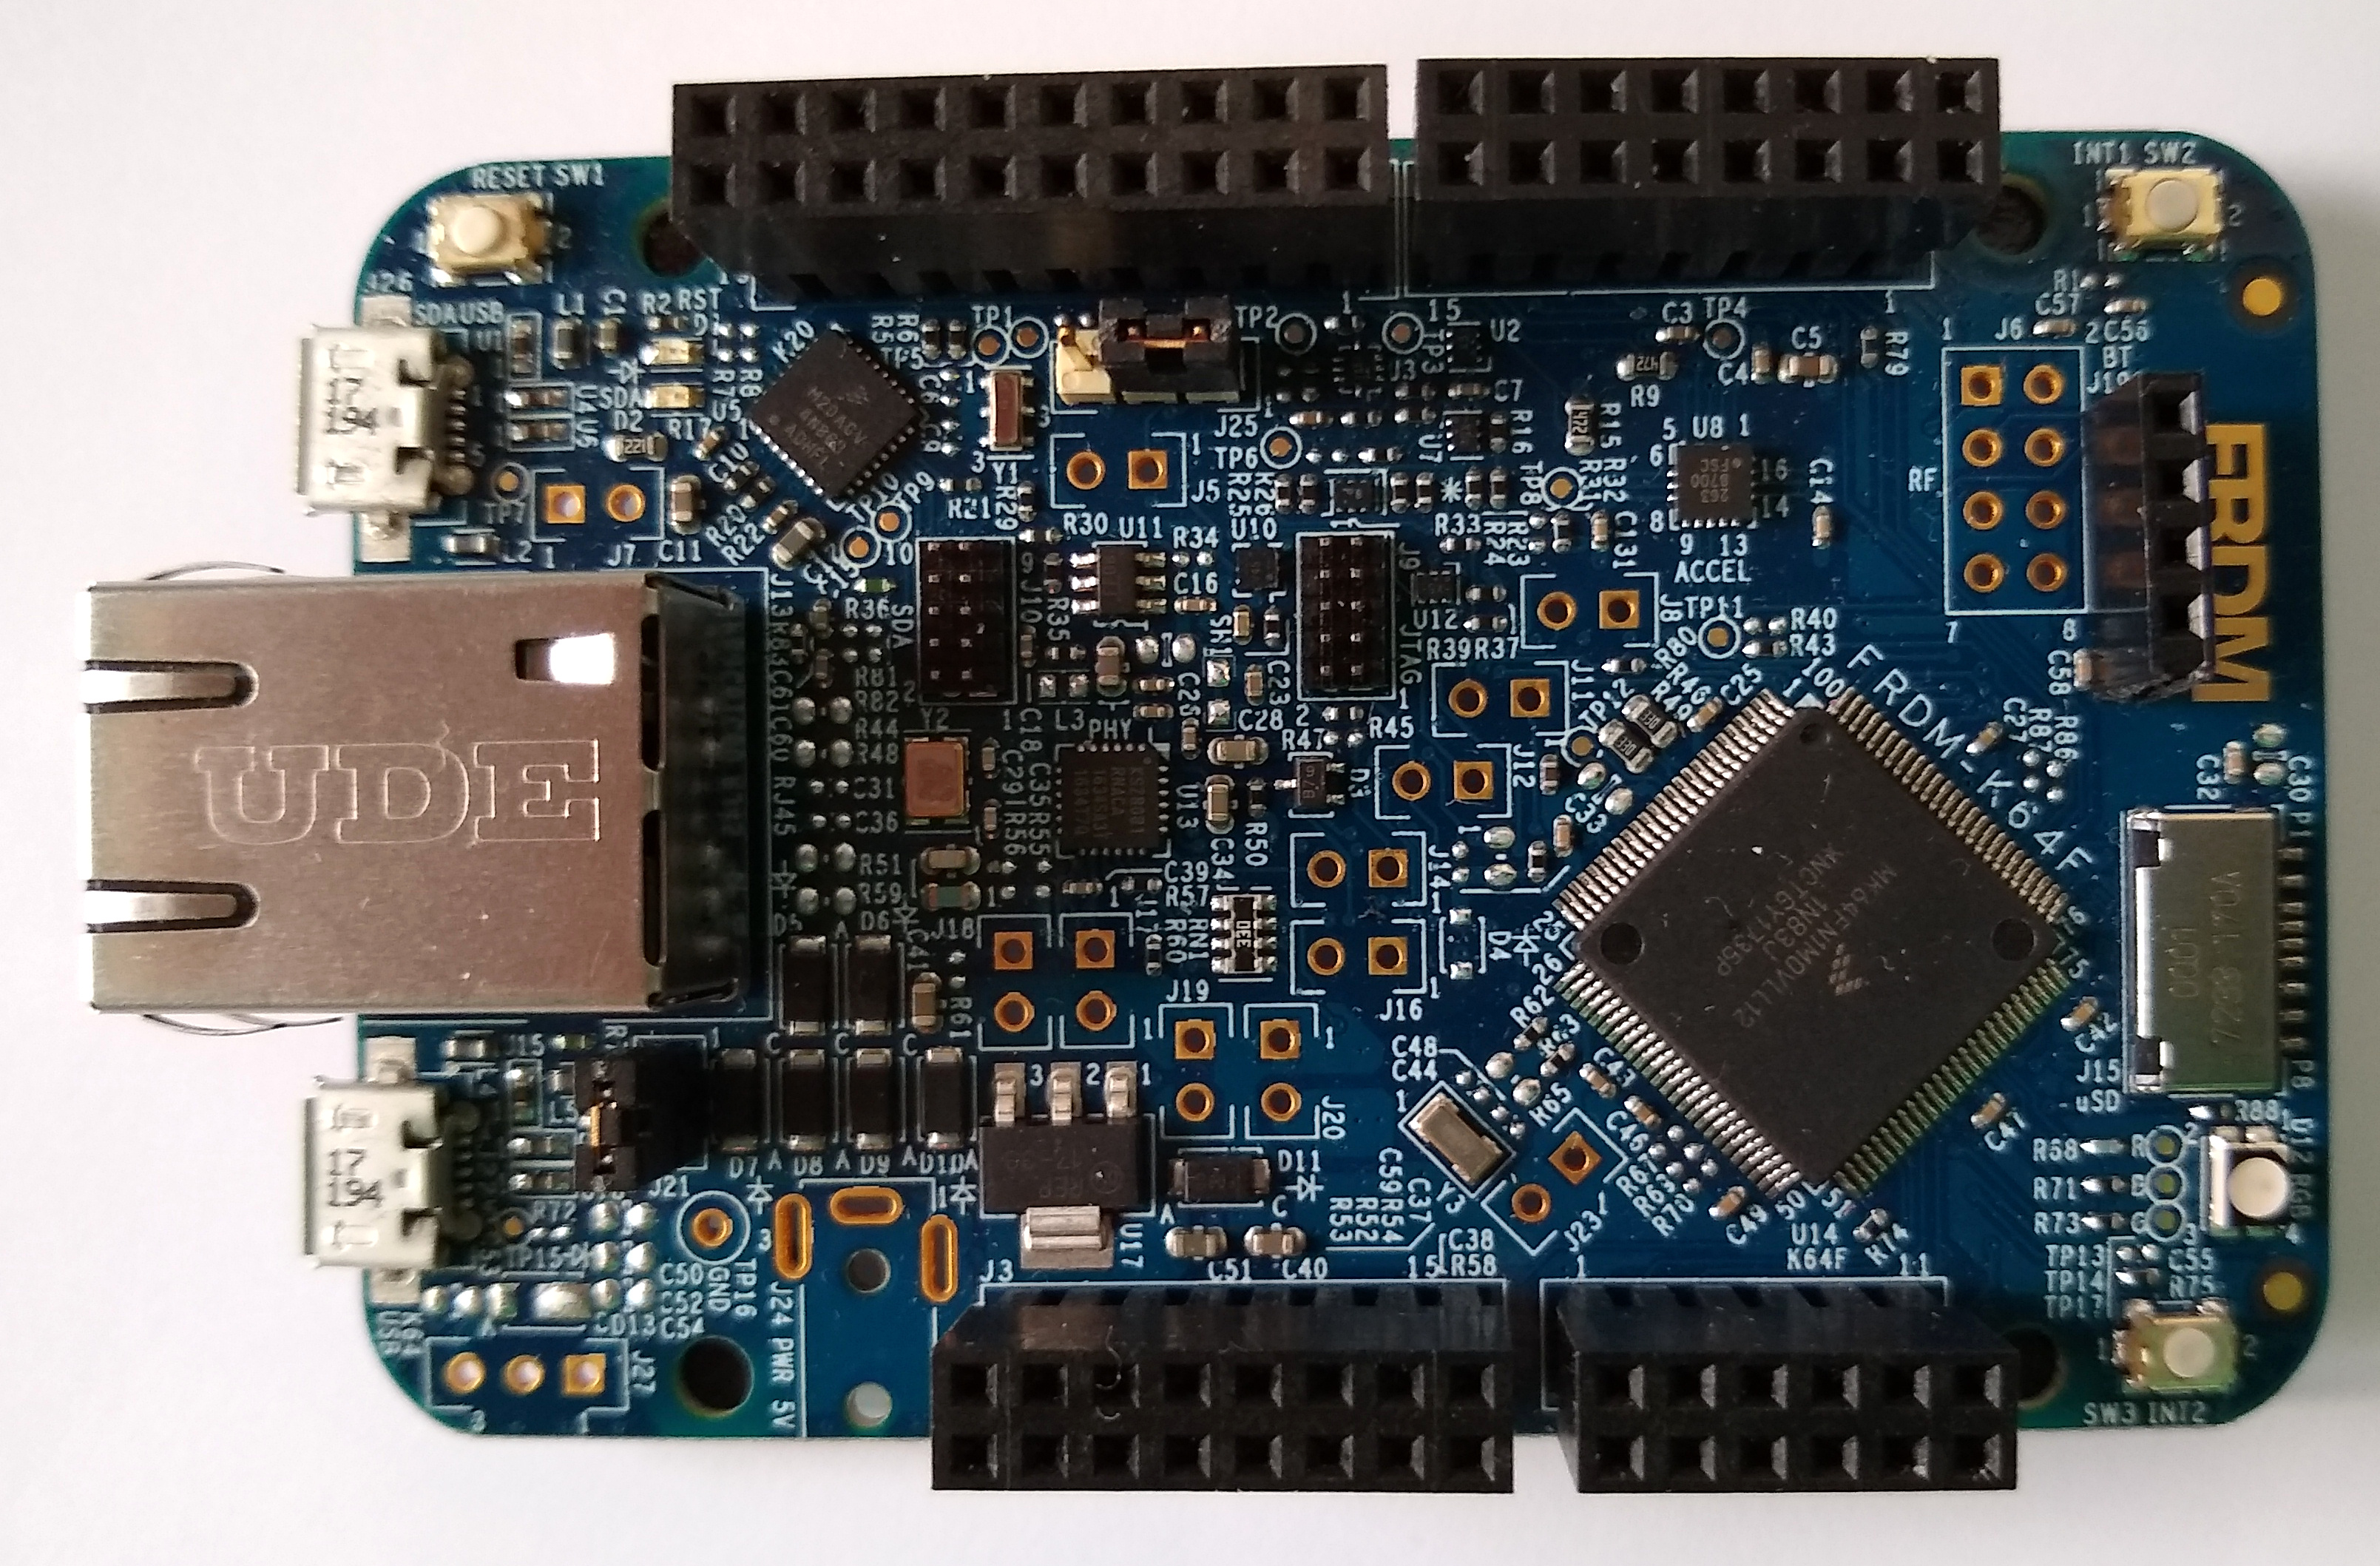
\includegraphics[width=0.7\textwidth]{k64f1.jpg}\par\vspace{0cm}
			\caption{FRDM-K64F development board}
		\end{figure}
		FRDM-K64F is a very capable development board manufactured by NXP Semiconductors with
		headquarters in Europe in Eindhoven, Netherlands and in North America in Austin, Texas. I chose this board due of my familiarity with it and of its abilities. This board and its cousin KL25Z were used throughout the course as part of the embedded systems modules.\\\\
		{\bfseries K64F development board specifications:}  	
		\begin{itemize}[topsep=4pt,itemsep=1pt]
			\item 120MHz ARM Cortex-M4 microcontroller
			\item 1MB Flash memory
			\item 256kB RAM
			\item Ethernet
			\item SDHC
			\item low-power
			\item FXOS8700CQ accelerometer and magnetometer 
			\item Add-on Bluetooth module: JY-MCU BT board V1.05
			\item RGB LED
			\item 2x user push buttons
			\item form-factor compatible with Arduino Uno Rev.3 pin layout
		\end{itemize}
		
		\subsection{Parallax 28821 Vibration motor}	
		\begin{wrapfigure}{r}{0.25\textwidth}
			\centering
			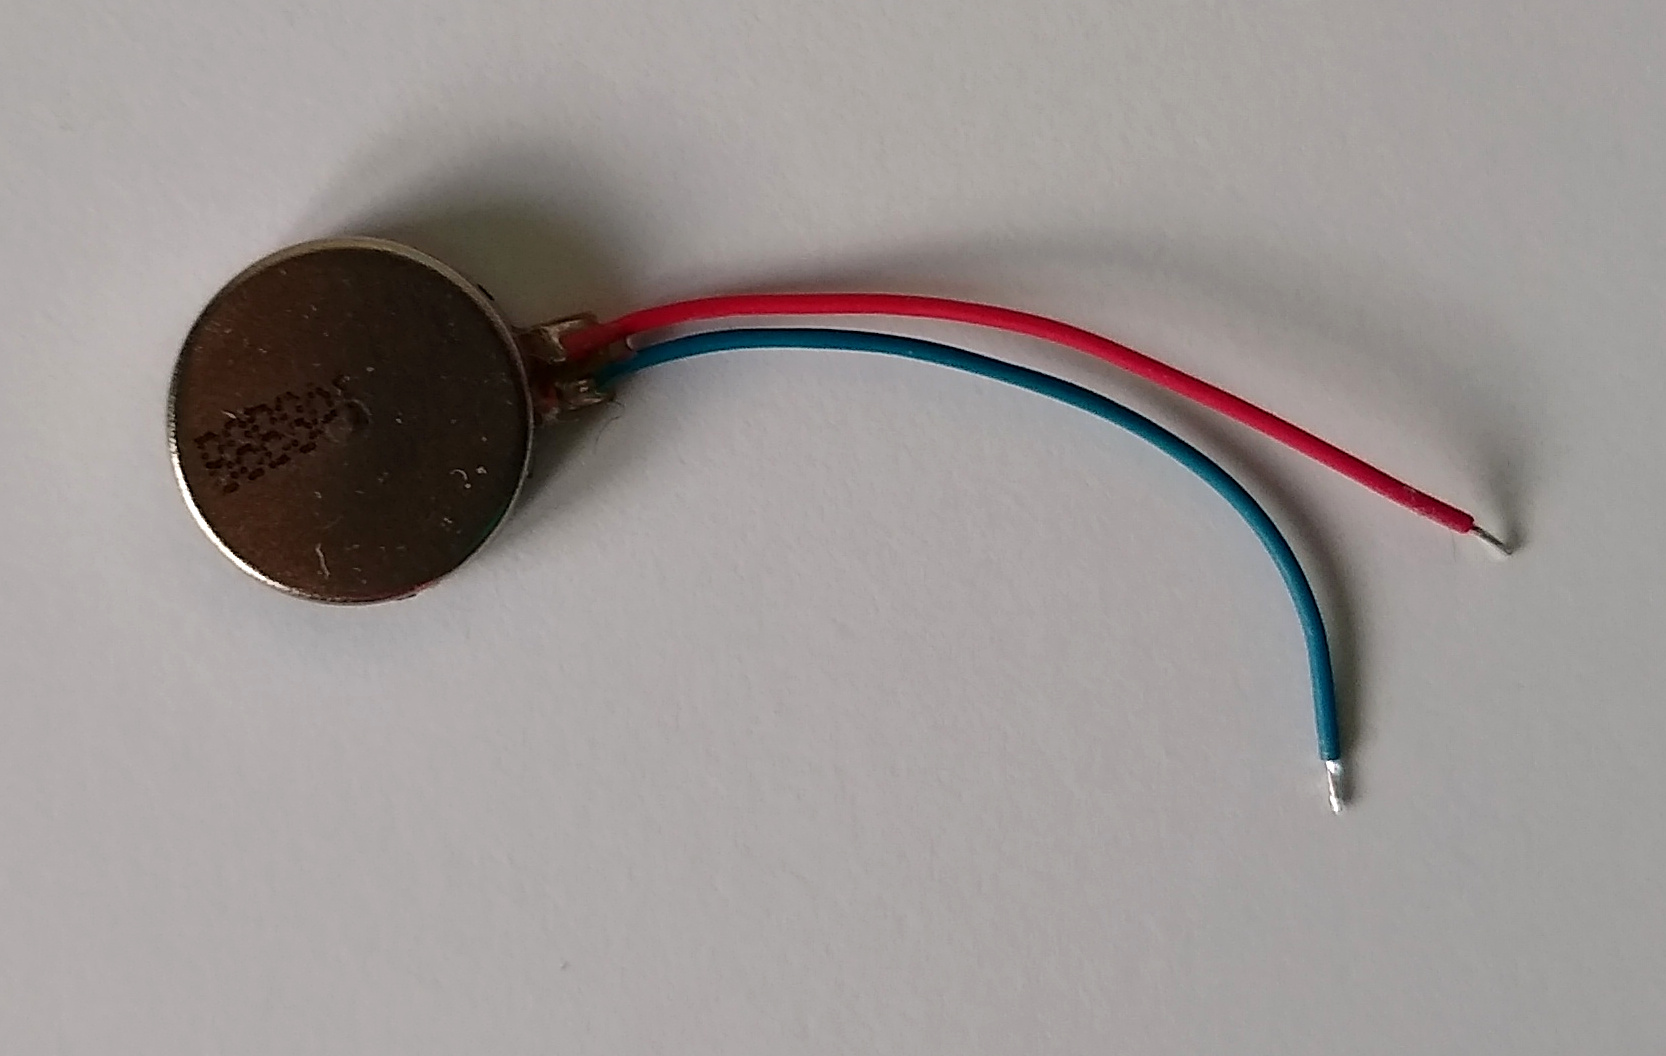
\includegraphics[width=0.2\textwidth]{parallax_vib_mot1.jpg}
			\caption{Parallax vibration motor}
		\end{wrapfigure}
		
		The vibration motor is used as a peripheral of the secondary device (bracelet) to gently and quietly wake the sleeping person up in the first stage of the overall wake-up process. The Parallax vibration motor seemed appropriate device for this task as it requires only 3V of power. However, the current it requires is quite high and cannot be supplied by the K64F thus an external supply has to be used.\\
		
		
        \begin{wrapfigure}{l}{0.4\textwidth}
         \centering
         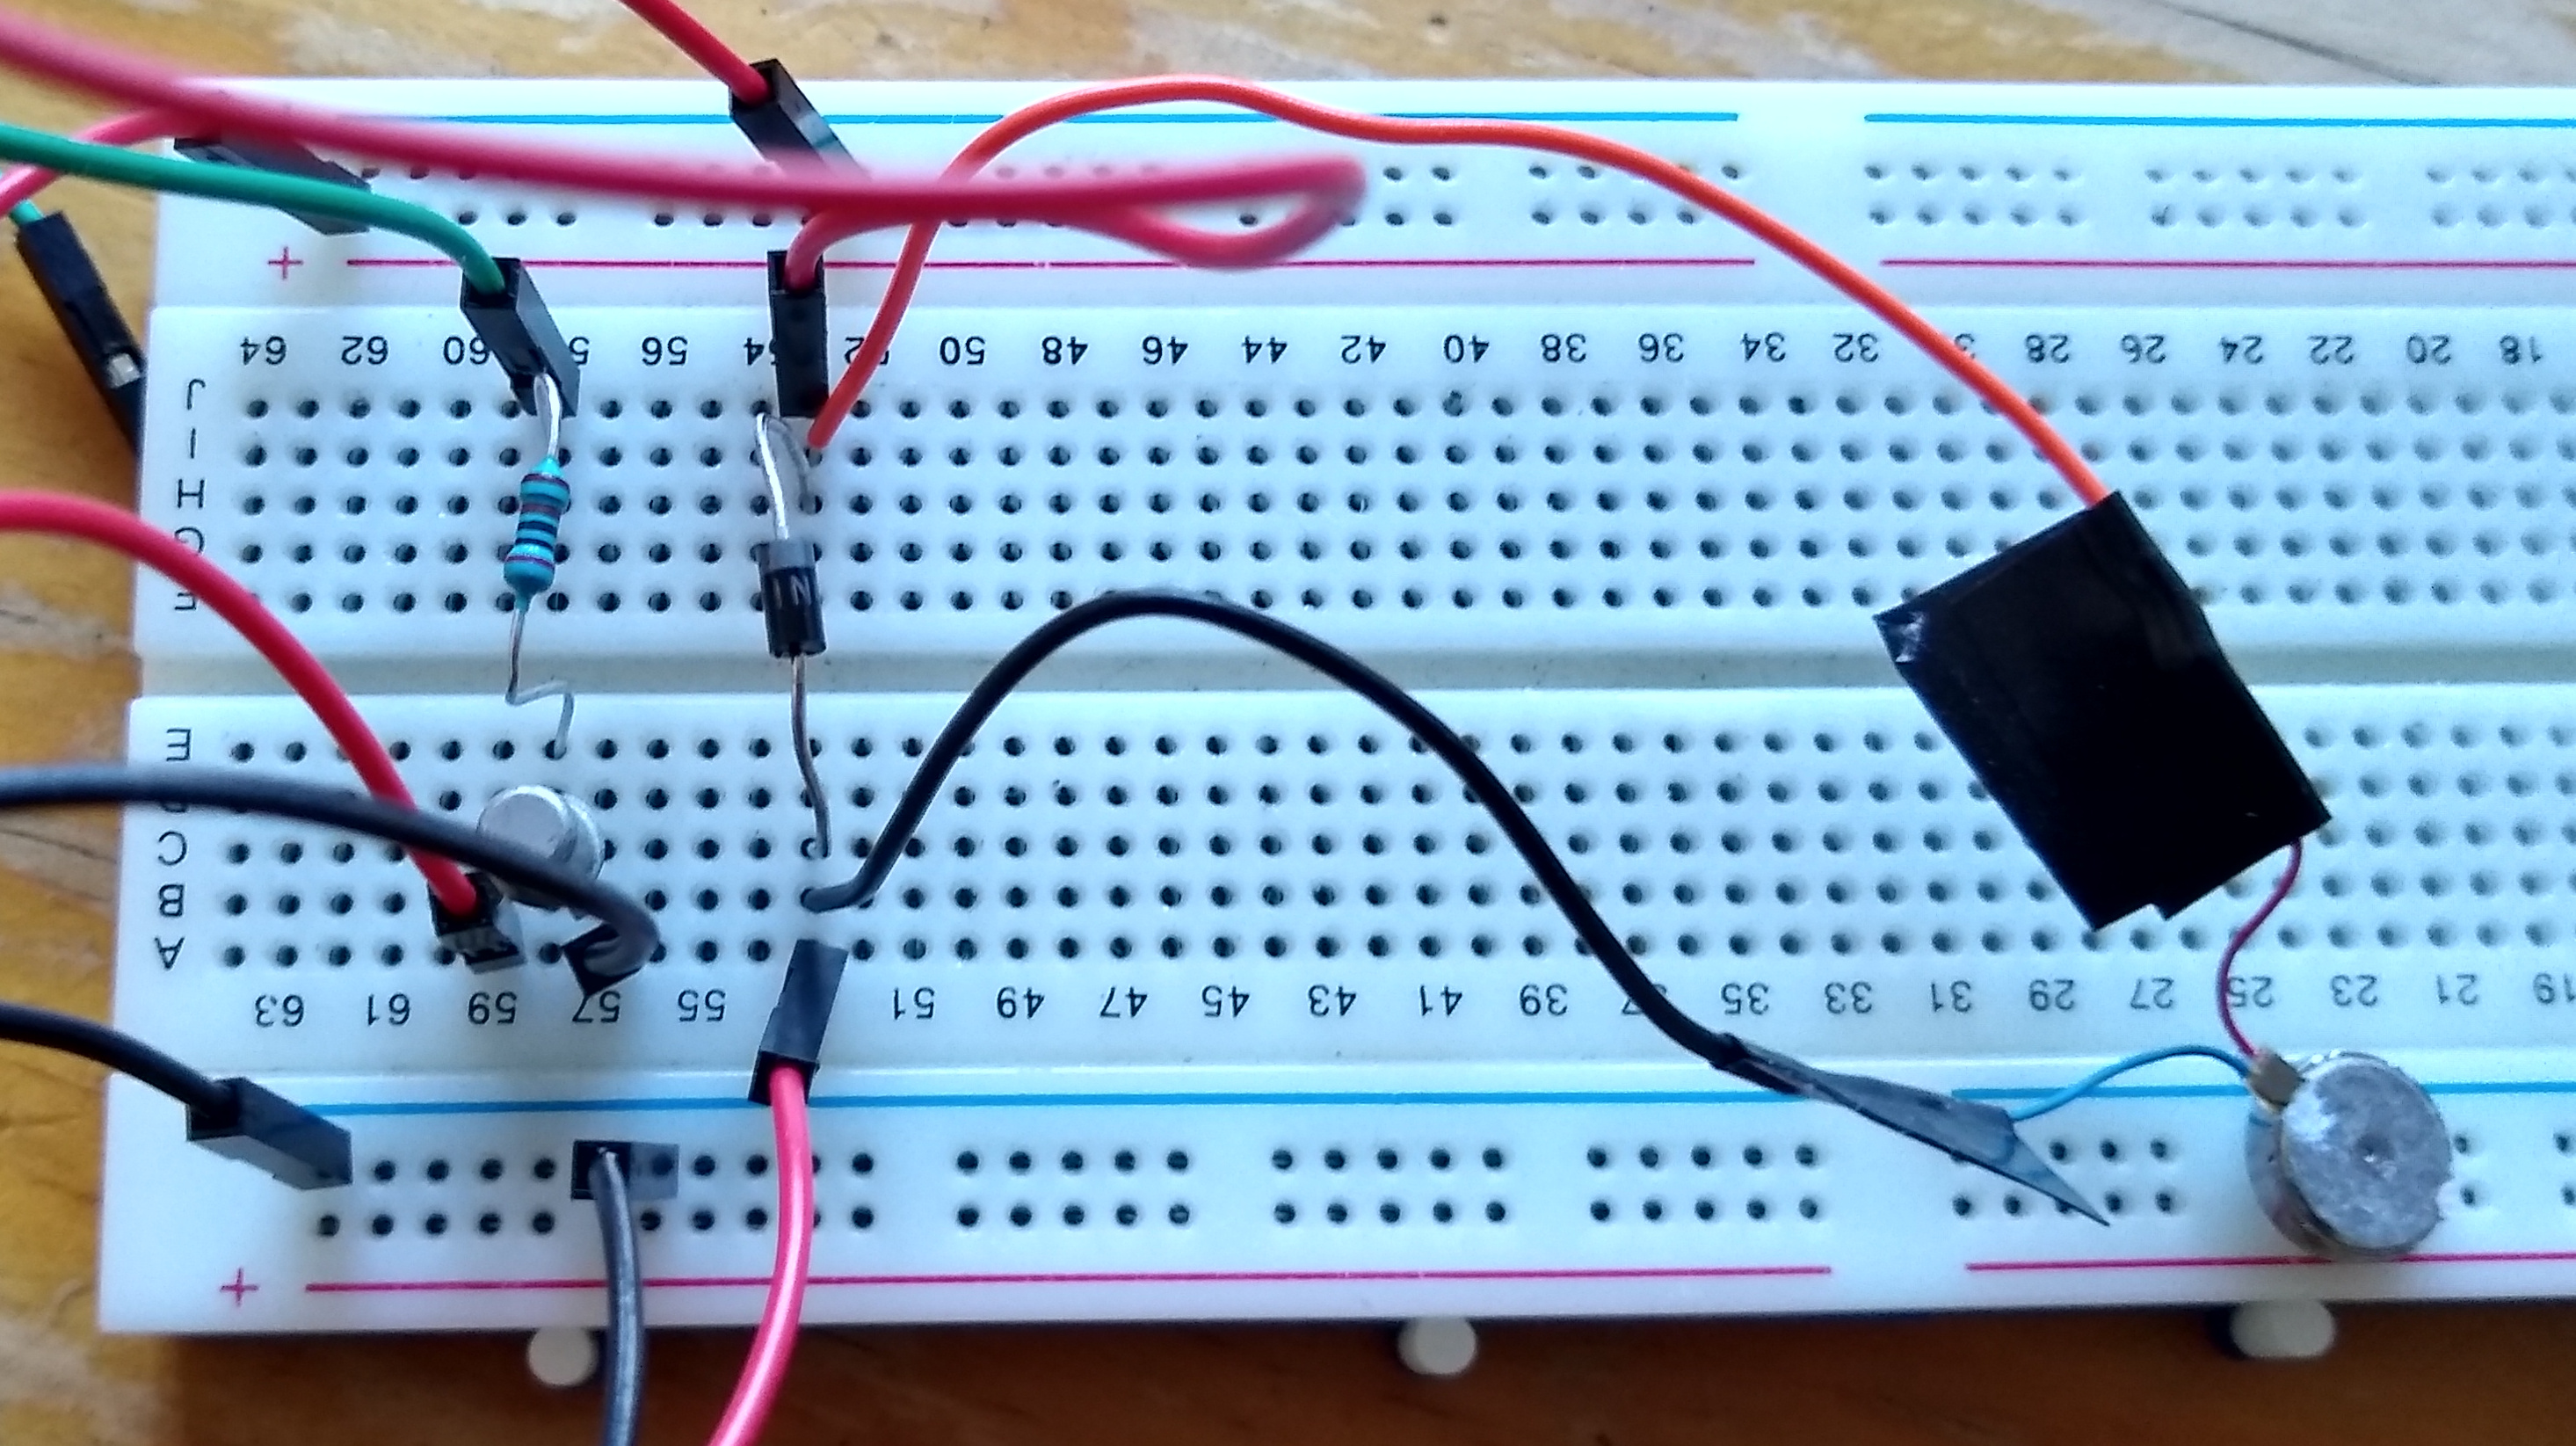
\includegraphics[width=0.35\textwidth]{circuit_proto.jpg}
         \caption{Prototyping}
        \end{wrapfigure}
        
        In order to being able to control this vibration motor, I had to assemble a simple circuit using BC108 transistor as a switch. I had to prototype this circuit first to ensure everything works as should and to prevent any damage to the microcontroller and then solder the circuit to a piece of protoboard.\\
        
		\begin{figure}[h]
			\centering
			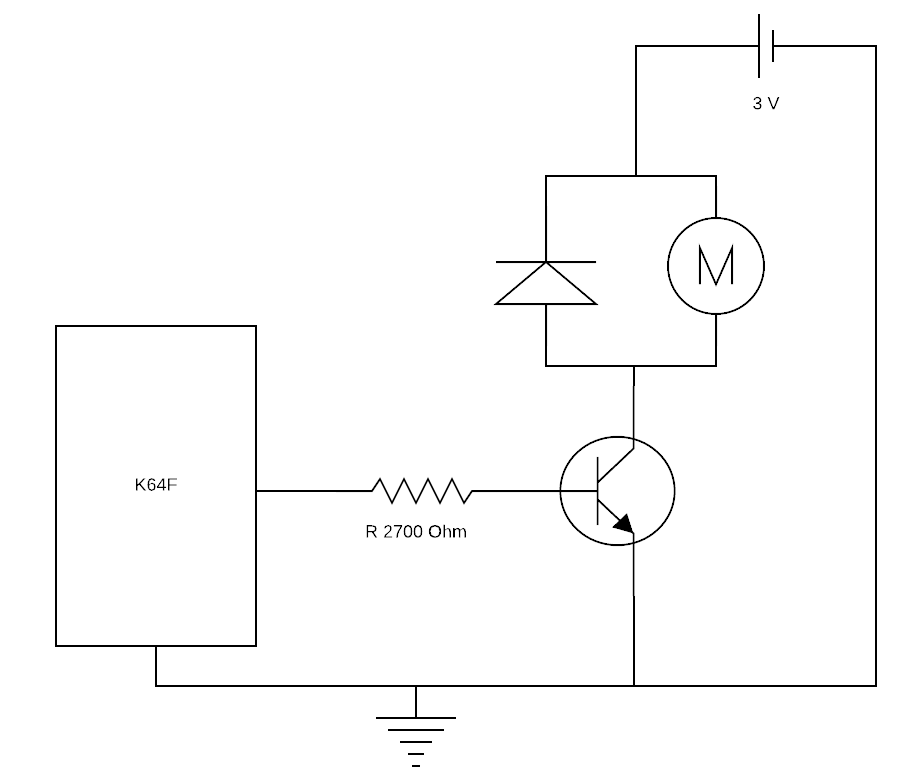
\includegraphics[scale=0.3]{motor_diag1.png}
			\caption{Vibration Motor Connection Diagram}
			\label{fig:vibMotorConnDiag}
		\end{figure}
        
		{\bfseries Motor specifications:}
		\begin{itemize}
			\item Rate voltage: 3.0V
			\item Rate current: 150mA
			\item Rate speed: 9,000r/min Min
			\item Starting voltage: 2.3V
		\end{itemize}
		
        \begin{figure}[h]
         \centering
         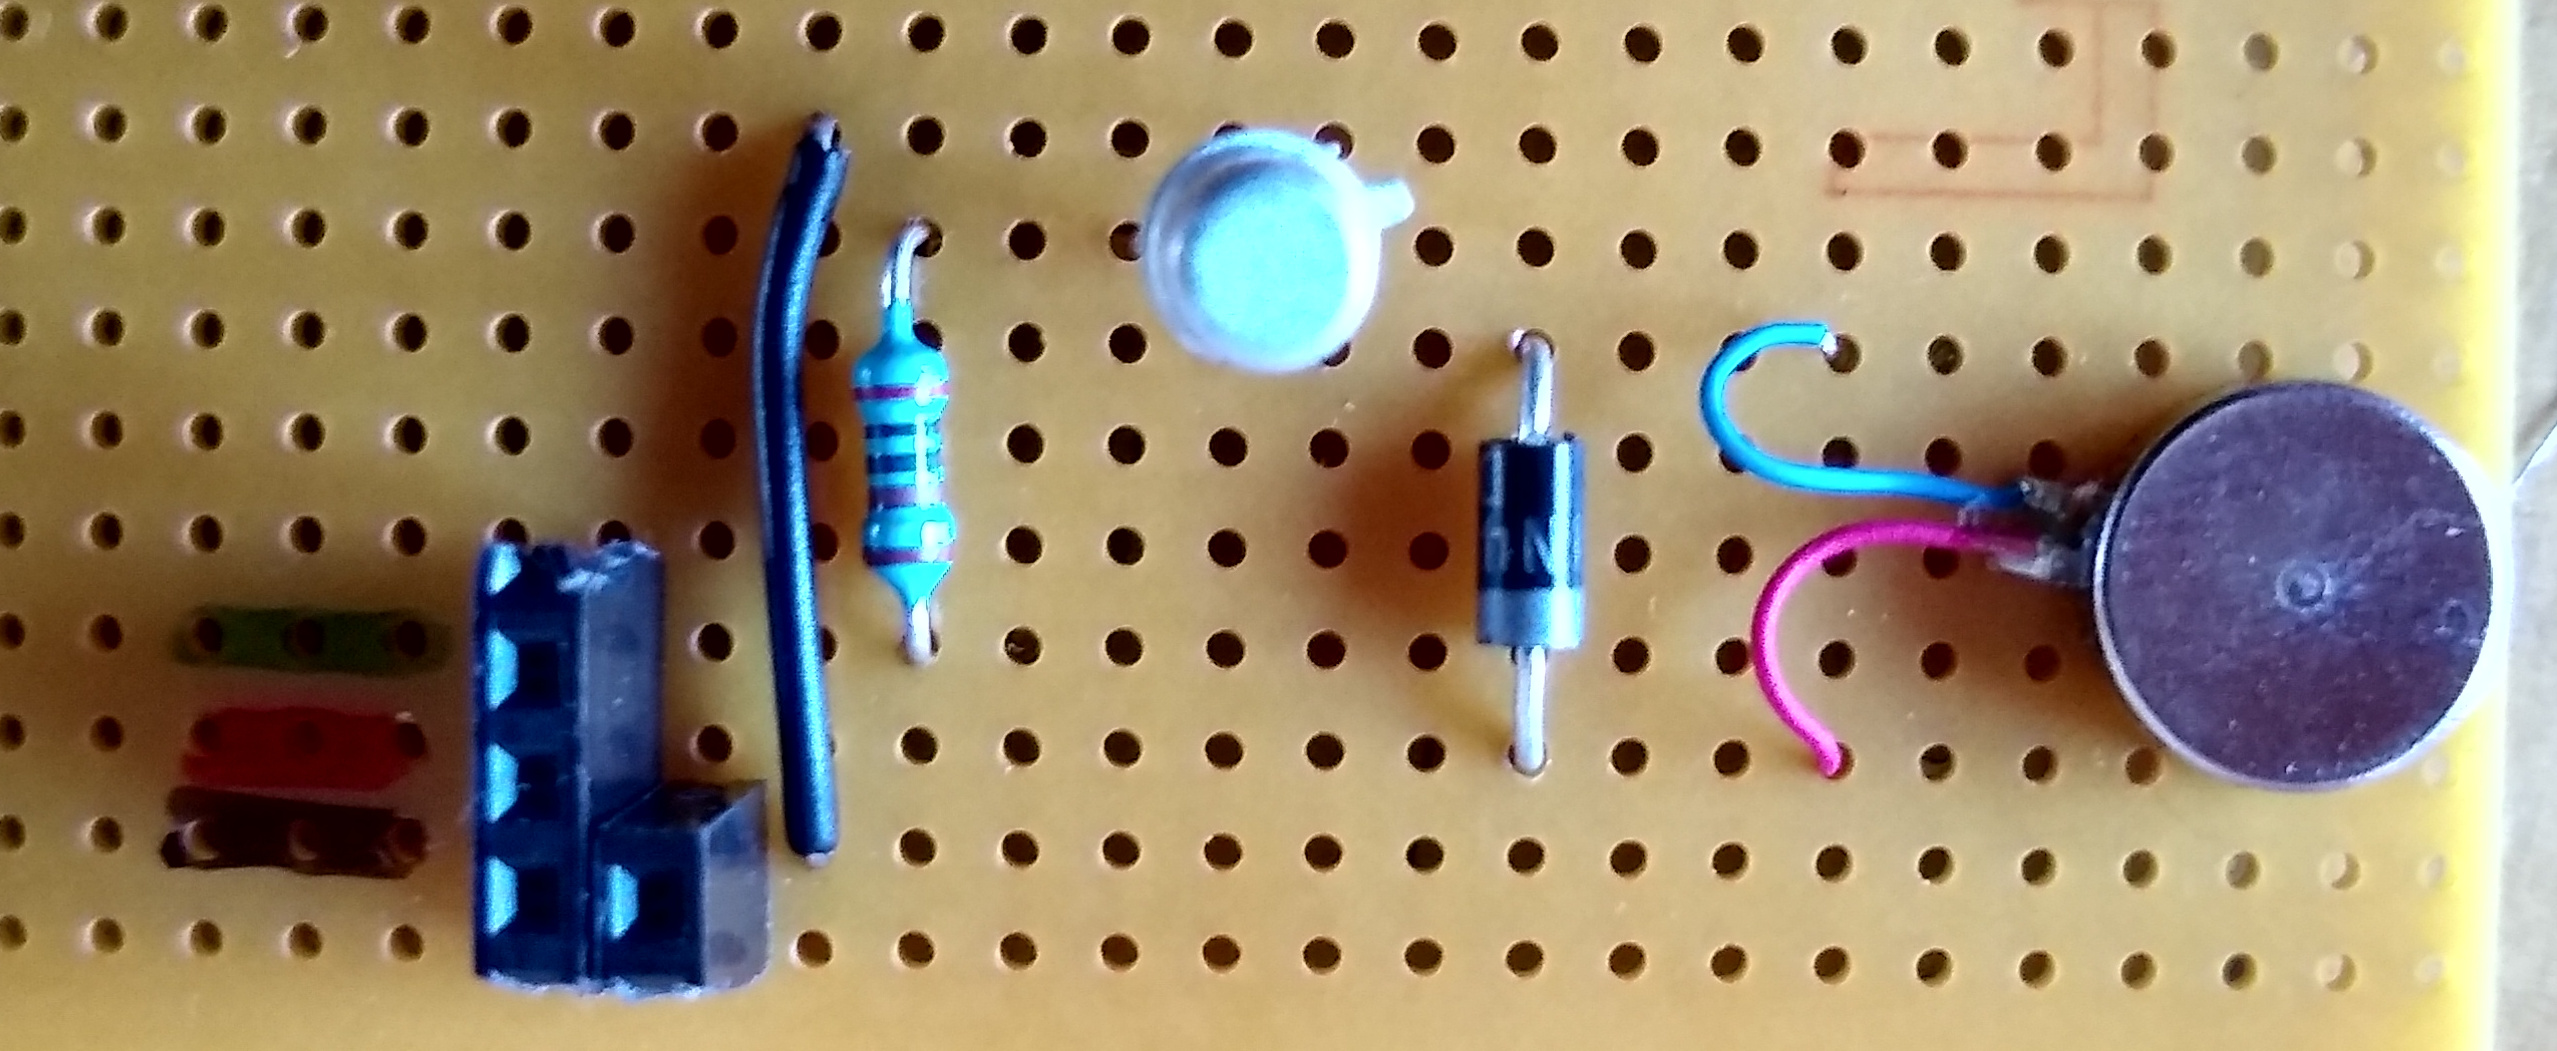
\includegraphics[width=0.5\textwidth]{circuit1.jpg}
         \caption{Vibration Motor Interfacing Circuit}
         \label{fig:vibMotIC}
        \end{figure}
		
		\newpage
		\subsection{Relay}
        \begin{wrapfigure}{L}{0.3\textwidth}
         \centering
         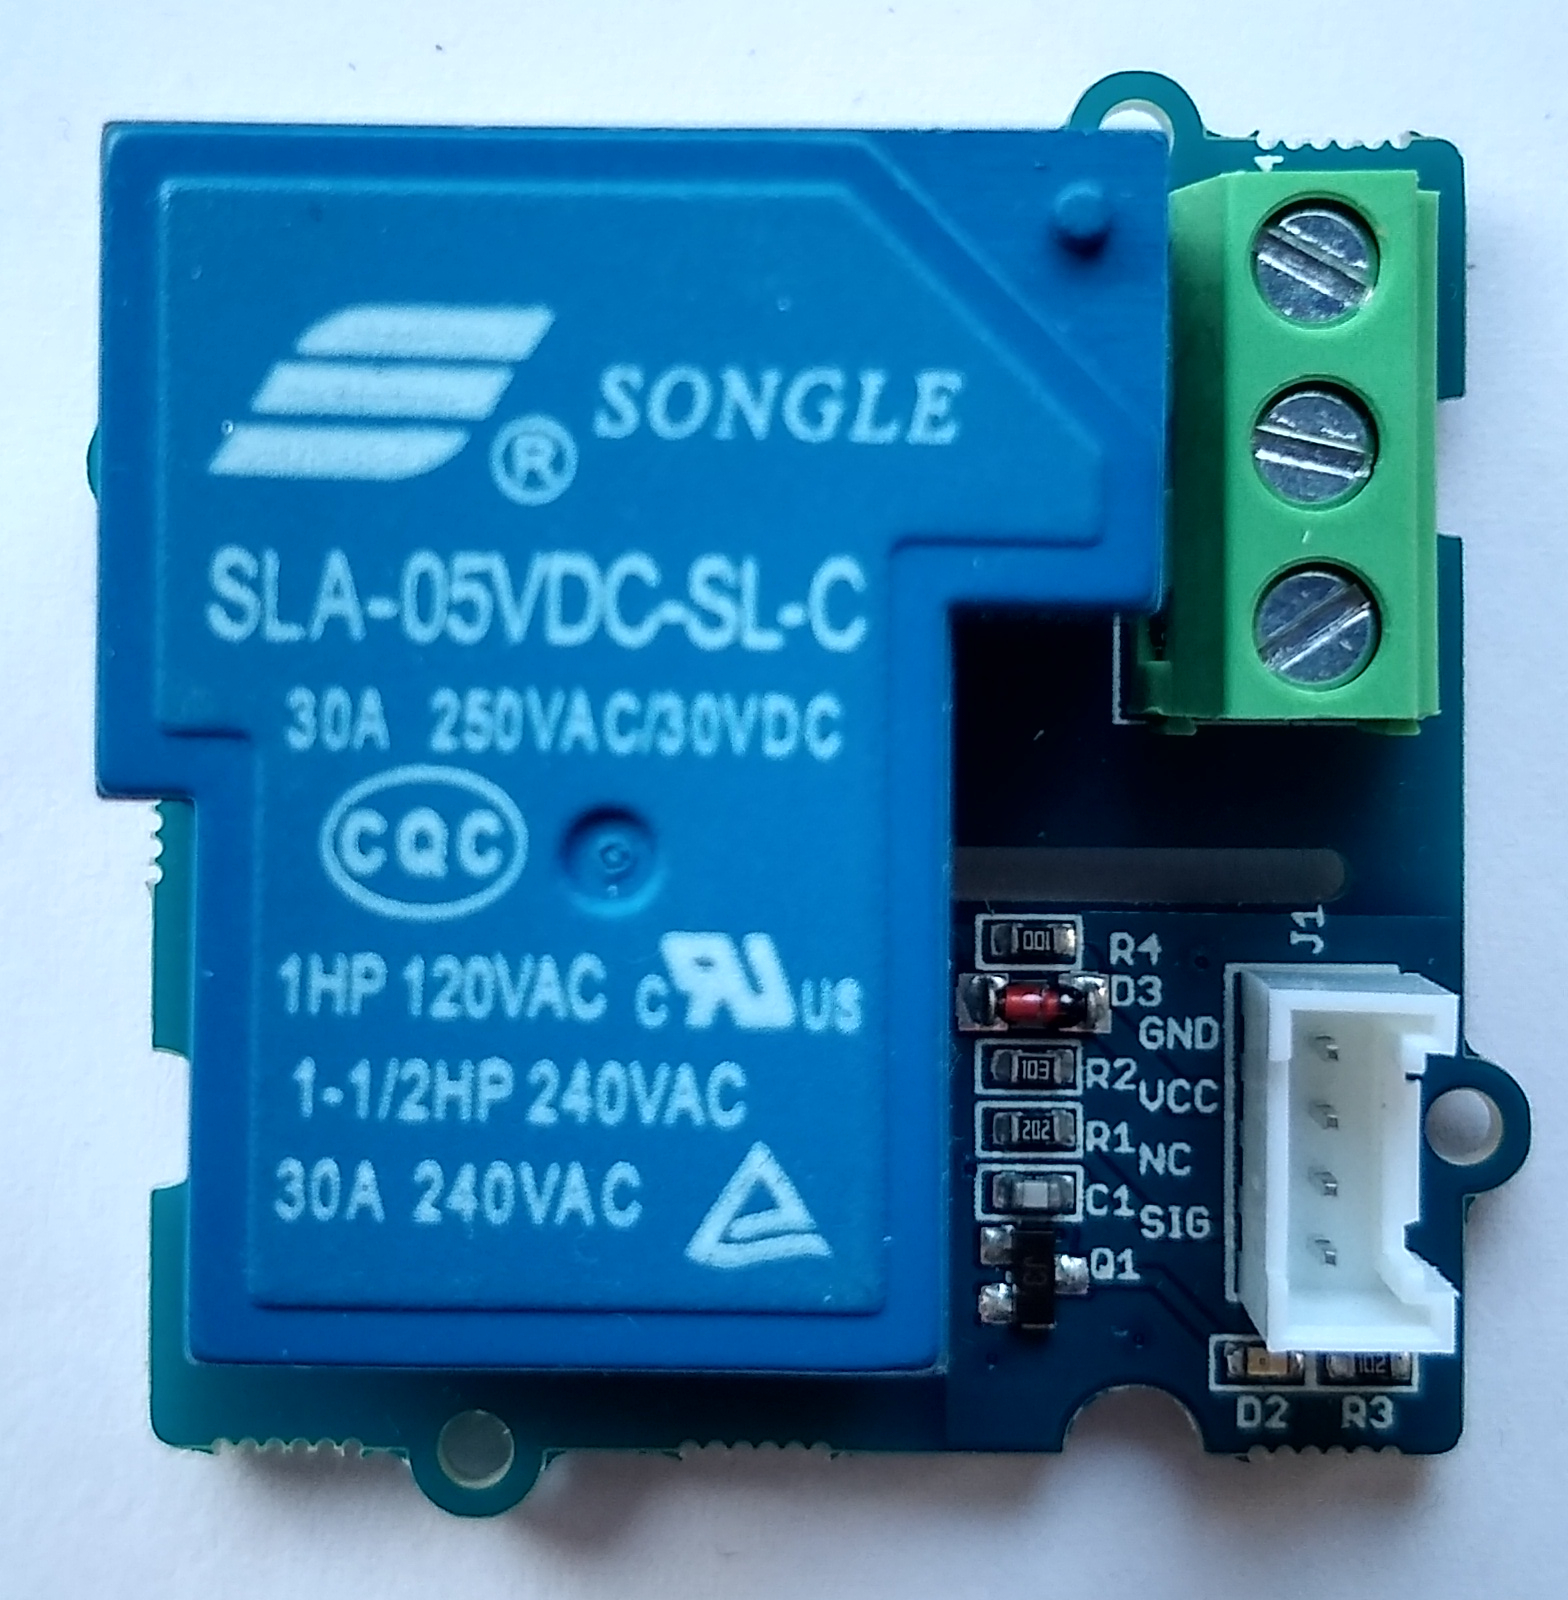
\includegraphics[width=0.25\textwidth]{relay1.jpg}
         \caption{Relay}
        \end{wrapfigure}
        
		The relay is used in the second stage of the wake-up process. It is connected to a lamp and is triggered when the first stage fails and more disruptive method is needed to wake the sleeping person up. To control this relay, a simple GPIO pin is used.\\\\\\\\\\\\

		\subsection{Buzzer}
        \begin{wrapfigure}[13]{R}{0.3\textwidth}
         \centering
         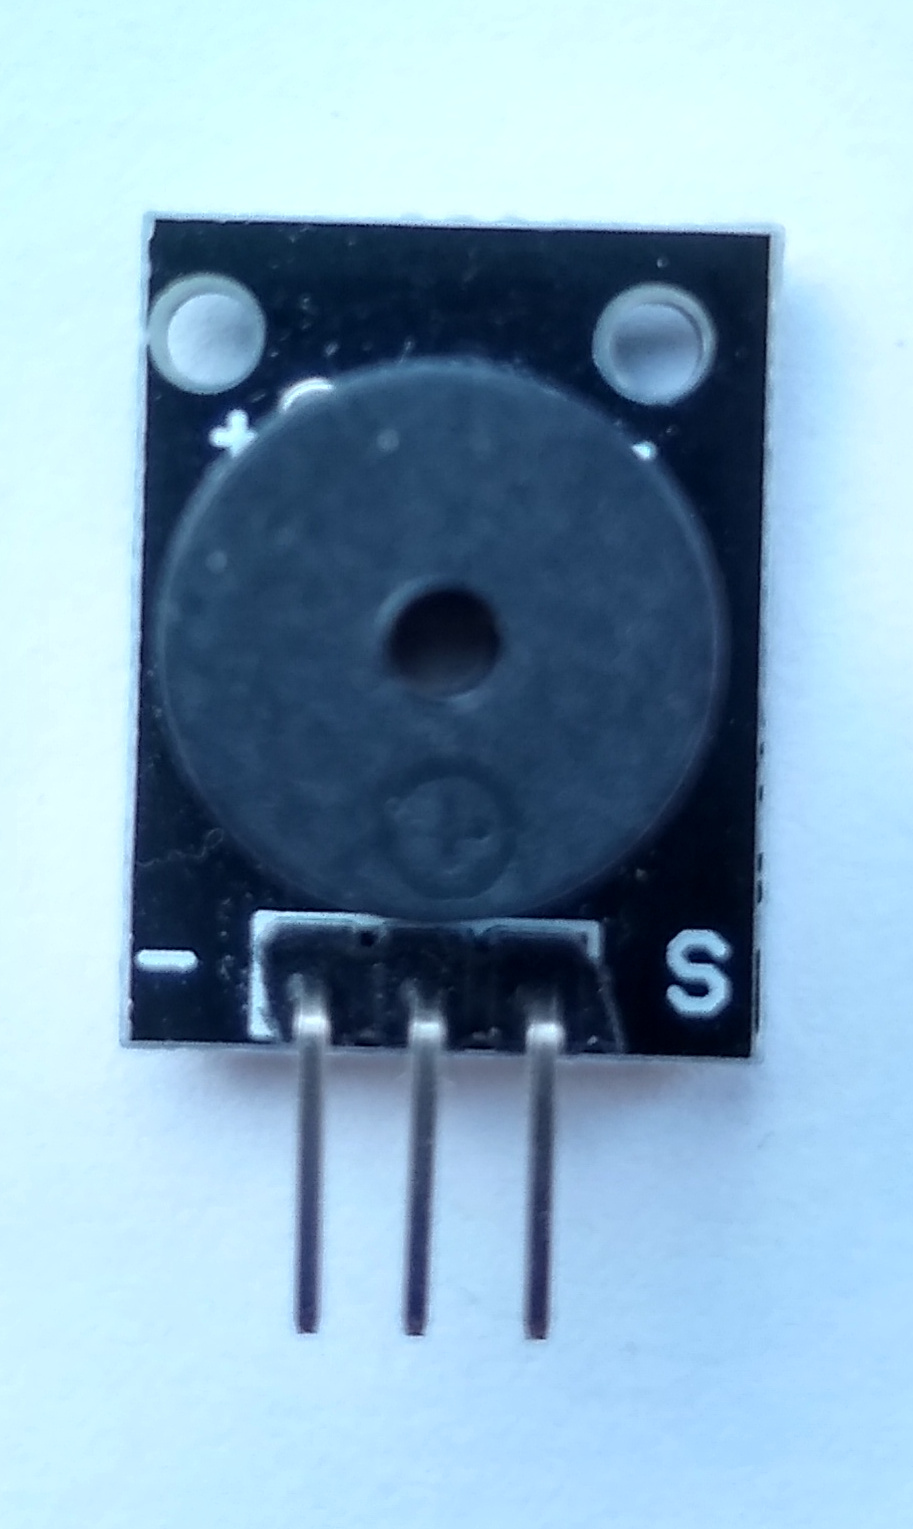
\includegraphics[width=0.25\textwidth]{buzzer1.jpg}
         \caption{Buzzer}
        \end{wrapfigure}
		The buzzer is used for the third stage of the wake-up process if the vibration motor or 
		relay fails to wake the sleeping person. This is a passive device and for the sound to be produced the Flex Timer Module of K64F is used to generate a PWM signal on the connected GPIO pin. This buzzer came as part of a multi-sensor kit I ordered for Arduino projects previously so I had it readily available for use in this project.\\\\
		
		\subsection{HC-05 Bluetooth module}
		
		\begin{wrapfigure}{L}{0.25\textwidth}
			\centering
			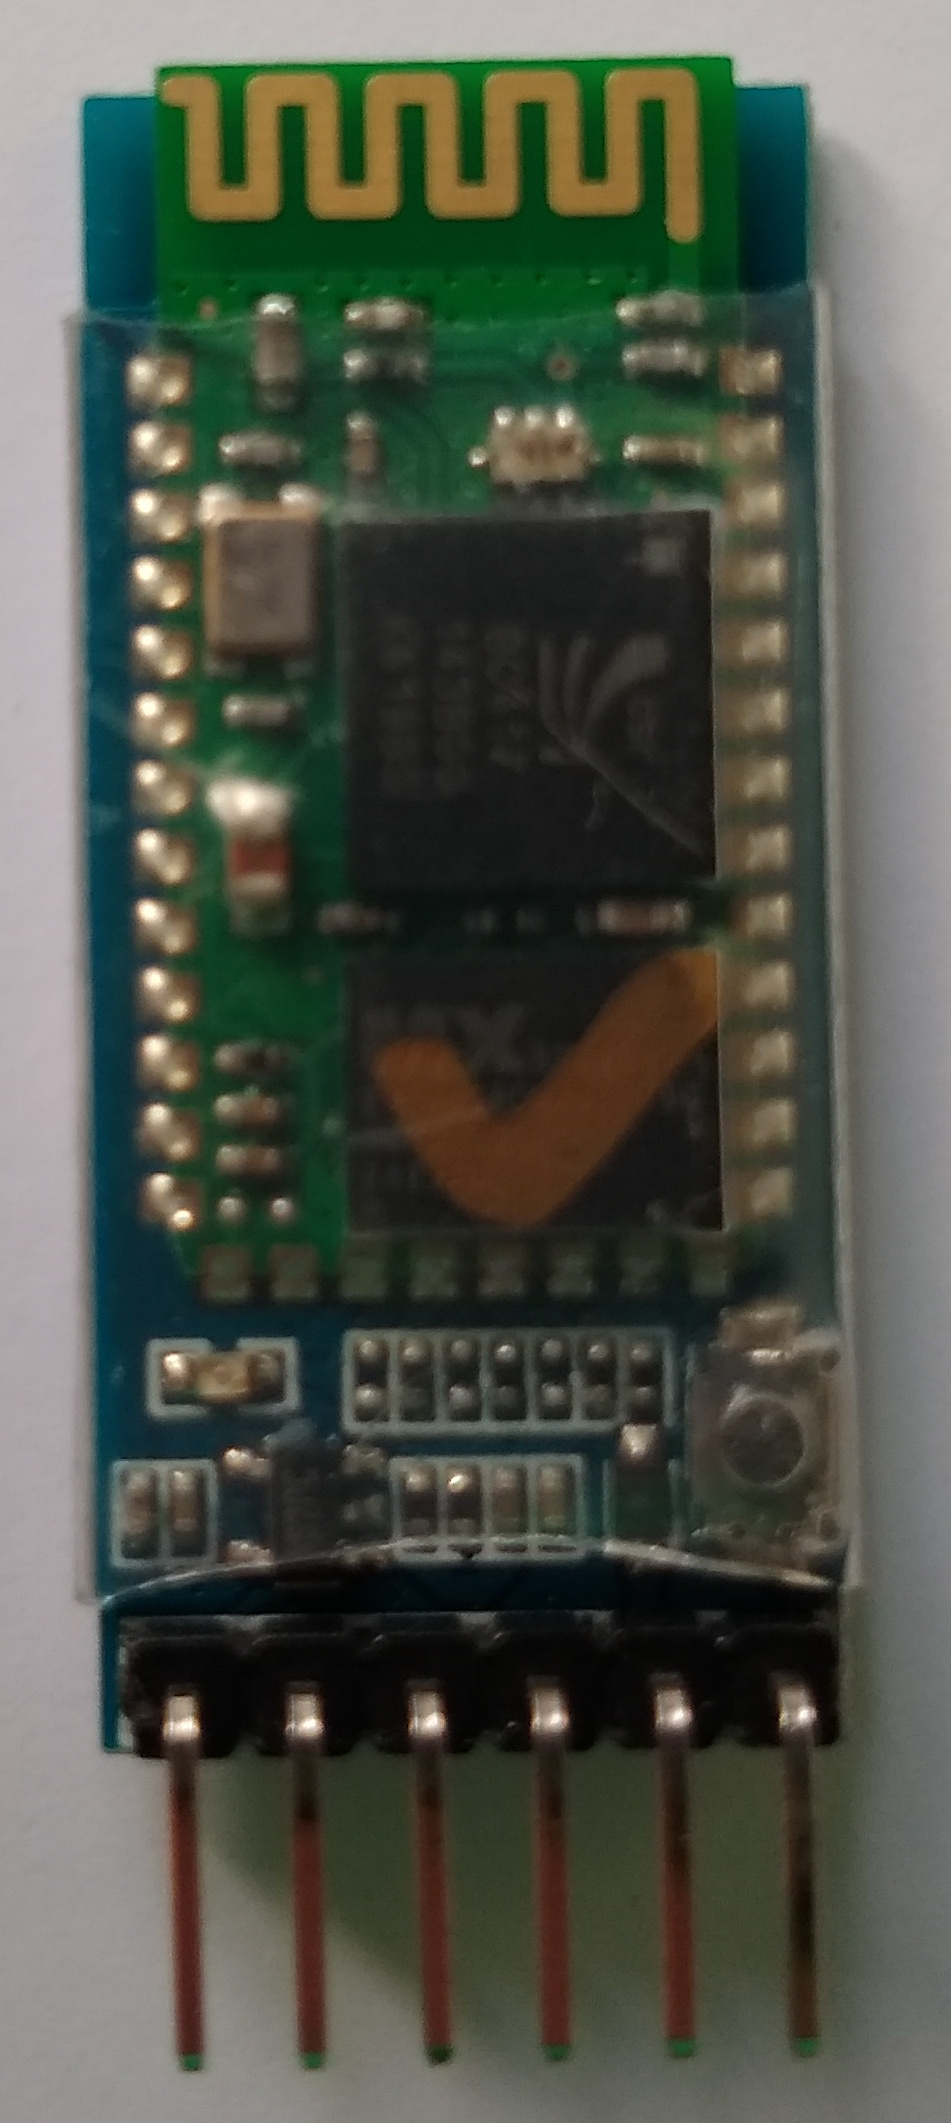
\includegraphics[scale=0.06]{hc-05_1.jpg}
			\caption[HC-05 Bluetooth module]{HC-05}
		\end{wrapfigure}

		HC-05 is a commonly used Bluetooth module often used with Arduino projects. The K64F development board supports  
		this module also. I have installed a small section of header pins to house this module. For my  
		project I am using two of these. One to communicate with the secondary device (bracelet) and the
		second one to communicate with the mobile phone.
		
		This module can operate as a master or as a slave. In case of the master device of Easysleep project, this Bluetooth module was configured as MASTER and module on the secondary device as the SLAVE. Second module had to be added to the Easysleep master to allow for communication with the mobile phone as these modules only support one-to-one communication.
		
		\subsubsection{Bluetooth module configuration}
		In order for the Bluetooth modules to communicate, both the master and the slave have to be configured in the same way. Additionally they also have to share the same password and have to be made aware of each other by whitelisting each others address through AT commands.\\ 
		
		To setup this configuration I used an FTDI cable and start the individual modules in AT mode. This is done by applying power to KEY pin prior to the VCC pin. To communicate with the Bluetooth modules and configure it in the way I needed, I have used {\bfseries Minicom}  - a Linux command line utility. I started this by issuing the following command upon starting the bluetooth module in AT mode.
		\begin{center}
		 minicom -b 38400 /dev/ttyUSB0
		\end{center}
		The following commands were used to setup the master device:
		\begin{itemize}
		 \item AT+UART=38400,0,0 (Baudrate, 1 stop-bit, no parity, default 8-bit mode)
		 \item AT+ROLE=1 (master)
		 \item AT+INQM=1,1,48
		 \item AT+PSWD=7777
		\end{itemize}
		Similar setup was used for the second device with the exception of the ROLE, where it needs to act as a slave device therefore the ROLE was defined as 0.
		\newpage
		
	\section{Software}
	{\bfseries Software used, Programming languages, IDEs, Software tools}\\\\
	Througout my project I used various software tools to develop C and Java code, as well as
	software to monitor the behaviour of the system. All the code for the embedded devices was developed on a Linux system, Android Studio was however too resource heavy for my laptop so I borrowed a lab computer with the permission of Michael Keaveney, the GMIT technician.
	
		\subsection{MCUXpresso}
		I used MCUXpresso 11.1 to develop code for K64F. This is an Eclipse based IDE tailored to suit NXP devices. There are lots of alternatives from other manufacturers such as Atollic Studio for STM32. I became familiar with this IDE during my time in GMIT as it 
		was used for code development in embedded systems classes. I also used this IDE during my work placement in Jaguar LandRover in 2019.\\
		
		The project uses Amazon FreeRTOS to efficiently manage various tasks of the system. This is an open-source real-time operating system and its usage greatly reduces the complexity of C code used for functionality of the system. A programmer can divide the code into smaller, easier to manage blocks known as tasks. A communication between those is facilitated through the usage of semaphores, notifications and queues.\\
		
		Prior to the commencement of work on the project I had to obtain the appropriate Software
		Development Kit. I did so, through the SDK Builder present on NXP website. This site allowed 
		me to select specific processor and middleware and generated an SDK package that I then 
		imported into the MCUXpresso. This package included all necessary drivers for various 
		peripherals present on the development board such as GPIO or FlexTimer driver.\\
		
		I also created a repository on Github to have a proven record of my work as required 
		by my supervisor and other lecturers (and also to have a safety net in case things went 
		wrong). This is an extremely useful tool to know and use. I was grateful to have the ability to 
		revert to previous revisions of my code throughout the development as on a small number of occassions, the  
		path I chose to steer the development proved unsuitable, and it would have been  
		impossible to revert the changes from memory.
		\newpage
	
		\subsection{Android Studio} 
		This integrated development environment was the best choice for the development of my mobile application. There are other options out there such as Eclipse IDE but the Android Studio is the most supported one and was actually used during my last semester in Mobile application development module - so I was already familiar with it.\\ 
		
		This IDE is developed by BrainJet, the studio behind the well known IntelliJ and one can really see the similarities of both environments. This is an advanced IDE with plenty of features fully supported by Google Inc.\\ 
		
		The idea behind this application was to allow the user to wirelessly control the Easysleep module. This communication allows the user to check Easysleep's time and date or configure those as well as request data of recent incidents and silence an ongoing alarm.\\
		
		During my project development I used a third party application that allowed me to send characters via Bluetooth to Easysleep and receive data back. I wanted to recreate this application in a way that would better suit the project.\\ 
		\newpage
		
		\subsection{Other}
		{\bfseries Additional software tools used}
		
            \subsubsection{SystemView}
            SystemView is a great tool developed by SEGGER for monitoring the behaviour of Real-time
            operating systems as well as interrupts. It is free to use. It requires J-Link to be either installed as a bootloader on the development board or a harware J-Link probe needs to be used. In my case I had access to the hardware version. In order for it to work fully, I had to cut two traces on the development board otherwise it would clash with the OpenSDA debugger and the code would not get uploaded to the memory.
                    
            \begin{figure}[h]
                \centering
                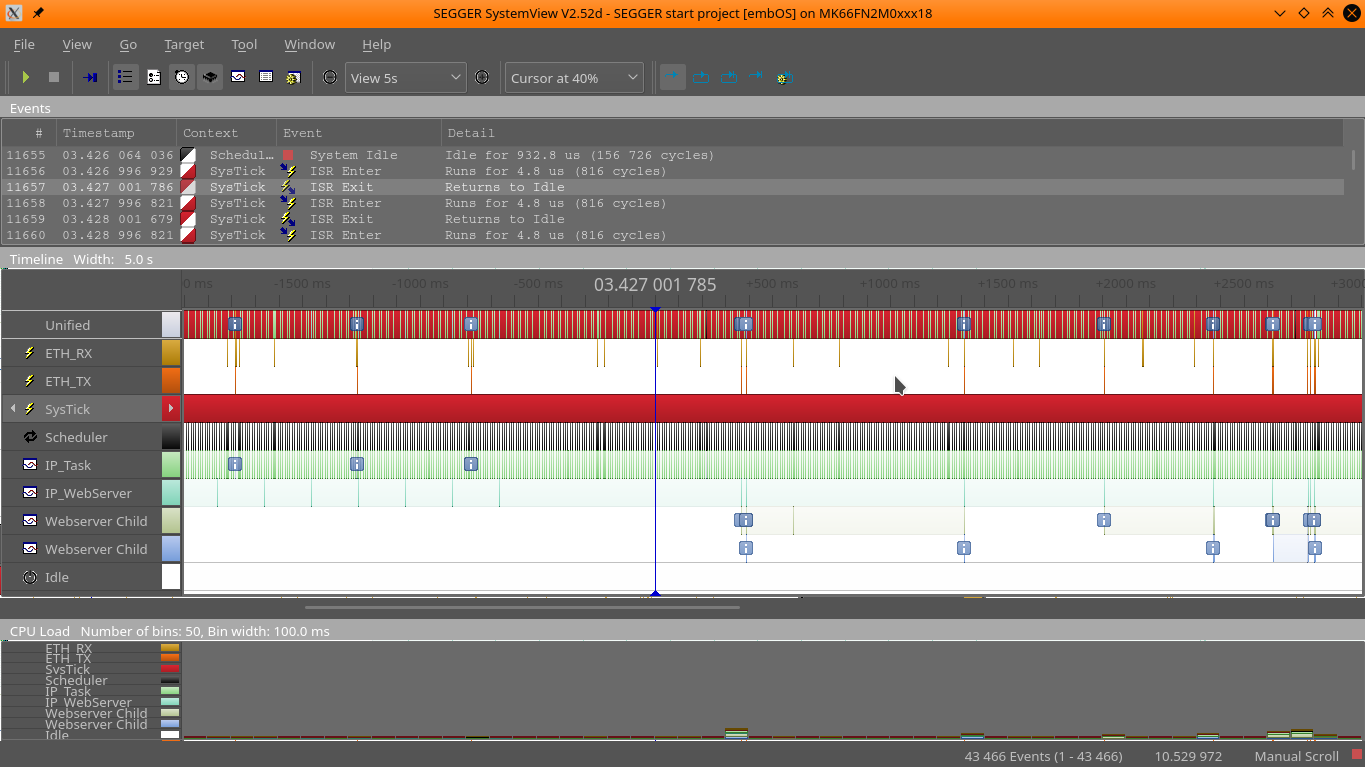
\includegraphics[width=0.7\textwidth]{systemview1}
                \caption{SystemView}
            \end{figure}
        
            \subsubsection{FreeRTOS}
            FreeRTOS is one of many real-time operating systems available. Other options include QNX, 
            ThreadX, embOS or Zephyr. Using a real-time operating system allows the programmer to 
            divide the functionality of the project into individual blocks that are easier to manage, 
            can communicate amongst themselves and maintain responsiveness. Real-time operating
            systems are often used in places where the functionality of a system is somewhat complex and a
            certain level of responsiveness is required (time-deterministic).
            
            \subsubsection{Pulseview}
            Pulseview is a Qt based logic analyzer. It is licensed under GNU GPLv.3. This software  
            allows the user to monitor the output of GPIO pins as well as decoding of various protocols,
            such as SPI or UART. This package is in the repositories of my Linux distribution so 
            installing it was as simple as typing a {\bfseries sudo apt install pulseview} into the command line and let the system to do the rest. This tool proved to be invaluable when 
            I was working with the buzzer and FlexTimer Module as it allowed me to monitor the output
            square wave.
            
            \begin{figure}[h]
                \centering
                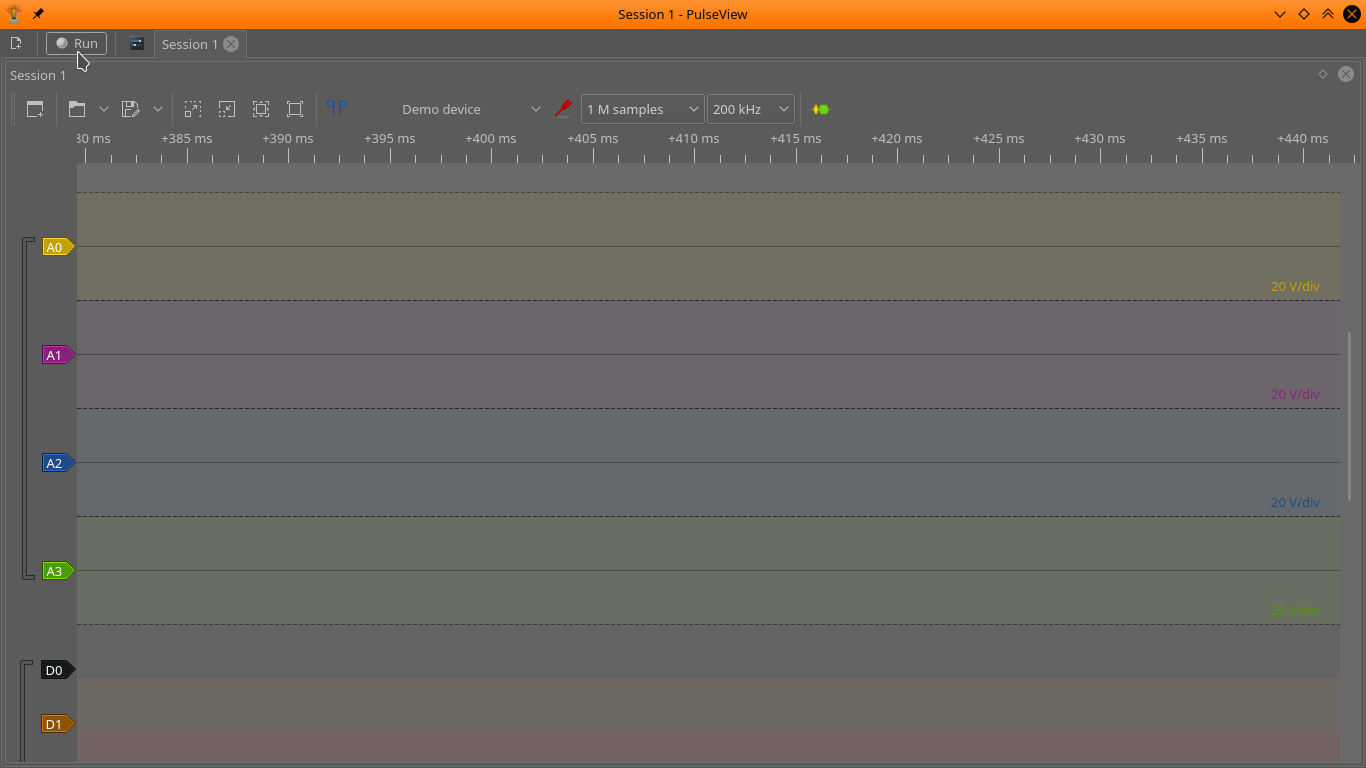
\includegraphics[width=0.7\textwidth]{pulseview}
                \caption{Pulseview}
            \end{figure}
        
            \subsubsection{Git/GitHub, gitk}
            Throughout the development of the C code for the embedded platform, as well as of the 
            Android application and this report, I used a Version Control System known as Git and 
            it's online counterpart GitHub. This allowed me to safely store my code, revert to 
            previous code revisions and work from different computers at school or at home.
            
            \subsubsection{Doxygen}
            Doxygen is a documentation generator widely used in software development companies. It
            allows user to generate documents describing code functionality by adhering 
            to certain code commenting standards.\\
            
            Doxygen is available for various programming languages. It comes with a large configuration 
            file that the user can adjust to suit the need of the project.
            
            \subsubsection{Project management software}
            project management software, BT configuration,
            \newpage
		
		\section{Code Development}
		{\bfseries Languages used, code development and examples}\\
		
		The programming languages that were used for the development for the code were C programming language and Java. C was used to program the two K64F embedded devices while Java was used for the Android application development.
		
		\subsection{K64F Master code development}
		\href{https://github.com/zedd-1983/project_journal/tree/bt2}{K64F Master Device code repository}\\
		I started developing the code for this device in early October 2019 and in parallell ordered few items via the technician in GMIT, i was able to proceed without having the ordered items to hand.  It was my intention to use FreeRTOS from the very beginning. This component was on the curriculum in the first semester of the final year at GMIT, however, I had already completed an online course in FreeRTOS the previous summer, so I was already familiar with it's concepts and inner workings. The Real-time Operating Systems module covered at GMIT in the final year, helped me to strengthen my understanding of the subject further.\\
		
		Through my online course, I became aware of the SystemView tool which allows the developer to monitor the behaviour of FreeRTOS tasks as well as of the interrupts. To use the software to it's full potential I had to order a SEGGER J-Link debugging probe so I could use the software's continuous recording capabilities and watch how the system behaves and reacts over time and to different interactions. Later on, I discovered that similar functionality can be achieved by upgrading the on-board debugger to J-Link version (in this case, the original on-board debugger of K64F is OpenSDA). If I didn't use the J-Link, I would be limited to recording of few seconds only, until the allocated SystemView buffer filled up. This would be problematic, because I would not be able to test everything this quickly. As a result, this exposed me to yet another tool that is commonly used in embedded software development and I hope to benefit from it in the future.\\
		
		In order to successfully use the J-Link Edu debugging probe, adjustments to the project had to be made first.
		First I had to download and extract SEGGER SystemView target sources and place them into the project folder. I had to setup the include paths in MCUXpresso so the header files and source files would be visible for the compiler. This is done via Projec -> Properties -> C/C++ build. Below is the directory structure of the SEGGER include files.
		\begin{figure}[h]
            \centering
            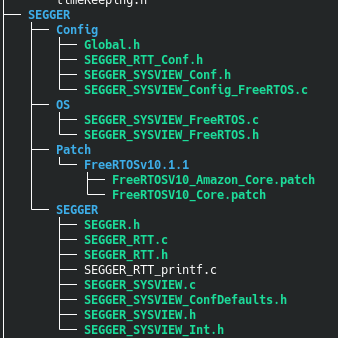
\includegraphics[scale=1]{SEGGER_directory_structure}
            \caption{SEGGER directory structure}
		\end{figure}
		All these files had to be included for the SystemView to work correctly, but additional adjustments had to be made to the code. First, a patch provided by SEGGER had to be applied to the FreeRTOS files in order to link the FreeRTOS with SEGGER target sources. The patching capability can be found in right-click menu under Team option. This will provide a list of files that would be patched and view of the actual changes for the developer to review.
		To continue with the integration of the SystemView I had to make changes to a number of files manually. First changes were added to {\bfseries FreeRTOSConfig.h} file.
		\begin{lstlisting}
        // FreeRTOSConfig.h
        #define INCLUDE_xTaskGetIdleTaskHandle 1
        #define INCLUDE_pxTaskGetStackStart 1
            .
            .
            .
        #include SEGGER_SYSVIEW_FreeRTOS.h
		\end{lstlisting}
		The {\bfseries SEGGER\_SYSVIEW\_FreeRTOS.h} has to be included at the end of the FreeRTOSConfig.h or above every include of FreeRTOS.h as it defines the trace macros to create SystemView events.\\
		The processor used has to be specified in {\bfseries SEGGER\_SYSVIEW\_Conf.h}. There are four macros to choose from defined in this file and as I used the ARM Cortex-M4 I had to redefine the SEGGER\_SYSVIEW\_CORE macro to SEGGER\_SYSVIEW\_CORE\_CM3.\\ 	
        I also had to define the size of the SystemView buffer in this file. By default this is set o 1024 Bytes but because the size of the RAM on K64F is 256kB I could afford to assign more to it so I have allocated 8kB of RAM. This would actually affect the amount of time that the data can be recorded by SystemView in Single-Shot mode (that is without the use of J-Link).
		\begin{lstlisting}
        // SEGGER_SYSVIEW_Conf.h
        #define SEGGER_SYSVIEW_CORE_OTHER   0 
        #define SEGGER_SYSVIEW_CORE_CM0     1 // Cortex-M0/M0+/M1
        #define SEGGER_SYSVIEW_CORE_CM3     2 // Cortex-M3/M4/M7
        #define SEGGER_SYSVIEW_CORE_RX      4 // Renesas RX
    
        #define SEGGER_SYSVIEW_RTT_BUFFER_SIZE (1024 * 8)
		\end{lstlisting}
		I also defined SystemView application name and SystemView device name in {\bfseries SEGGER\_SYSVIEW\_Config\_FreeRTOS.c} as well as SystemView RAM base address which on this microcontroller is at address 0x20000000.
		\begin{lstlisting}
        // SEGGER_SYSVIEW_Config_FreeRTOS.c
        #define SYSVIEW_APP_NAME         "Easysleep - Dev1_moisture_detection"
        #define SYSVIEW_DEVICE_NAME      "MK64FN1M0XXX12"
        #define SYSVIEW_RAM_BASE         (0x20000000)
		\end{lstlisting}
        Next step was to enable the ARM Cortex Mx Cycle Counter which is done by enabling the Current PC Sampler Cycle Count Register of Data Watchpoint and Trace unit {\bfseries DWT\_CYCCNT} as it is disabled by default. This register holds the number of core cycles and this can be used to measure elapsed execution time. In SystemView, it provides the timestamp of application events since the start of the program.
        To enable this register the following code has to be written to the top of the main.c function. It sets the zeroth bit to 1, in DWT\_CTRL register enabling the DWT\_CYCCNT register.
        \begin{lstlisting}
        DWT->CTRL |= (1 << 0);
        \end{lstlisting}
        Final step to enable recording of the application events is to include two SEGGER functions in the main.c file before the creation of any tasks or of the FreeRTOS scheduler. If either of these two functions isn't included, the recording won't start.
        \begin{lstlisting}
        SEGGER_SYSVIEW_Conf();
        SEGGER_SYSVIEW_Start();
        \end{lstlisting}
        This would conclude the initial setup of the SystemView. This tool is very powerful and useful especially when the system gets more complex. Having a visual representation of the systems behaviour can be at times very helpful.
        
        \subsubsection*{main()}
        Three tasks are created at the beginning of the program and a FreeRTOS scheduler is started. These are the moisture detection task, btTask and phoneBTTask.
        \begin{lstlisting}[label={lst:itCreation}, caption=Initial Task Creation]
        xTaskCreate(mainTask, "Main Task", configMINIMAL_STACK_SIZE + 1000, NULL, 2, &mainTaskHandle);
        xTaskCreate(btTask, "BT Task", configMINIMAL_STACK_SIZE + 50, NULL, 2, &btTaskHandle);
        xTaskCreate(phoneBTTask, "Phone Bluetooth Task", configMINIMAL_STACK_SIZE + 300, NULL, 2, &phoneBTTaskHandle);
        \end{lstlisting}
        In order to allow for some data transfer between tasks I had to create a number of FreeRTOS queues and initialize FreeRTOS semaphores (listing ~\ref{lst:semQue}) in following manner. 
        \begin{lstlisting}[label={lst:semQue}, caption=Semaphores and Queues]
        recordsForThePhoneQ = xQueueCreate(1, (sizeof(char[23]) * 3));
            .
            .
            .
        moistureDetectionSemphr = xSemaphoreCreateBinary();
        \end{lstlisting}
        
        \subsubsection*{mainTask()}
        {\bfseries mainTask} is responsible for recording the moisture detection events as well as creating some of the other tasks as needed. When the mainTask receives a notification from the external interrupt, it requests current date and time from the RTC module and records this. It also sets up an alarm interrupt to be triggered on the subsequent night just few minutes prior to the recorded time of the event.  
        
        Each of these tasks is assigned a memory stack size that it can use for storage of it's local variables. As the mainTask is used later for creation of other tasks, it was  necessary to assign a larger area of memory to it. Additionally, each of the tasks is assigned a priority value. In a  pre-emptive realtime operating system, the task with the highest priority runs. Other tasks can only run if the task with higher priority has been suspended or deleted.\\
        
        \subsubsection*{Moisture detection}
        I have also used a number of external interrupts in this system. An external interrupt is triggered currently by pressing a Button2 on the K64F device to simulate the moisture detection event. By nature, system interrupts have higher priorities to the FreeRTOS ones, therefore, they can interrupt running tasks. In this case, a FreeRTOS semaphore is given to the mainTask which upon taking it (listing ~\ref{lst:mdSemaphore}) records the events time and date and store it in an array as a string using a {\bfseries convertRecordToString()} function (listing ~\ref{lst:crtString}). This array can hold up to 10 events.\\
        
        \begin{figure}[h]
         \centering
         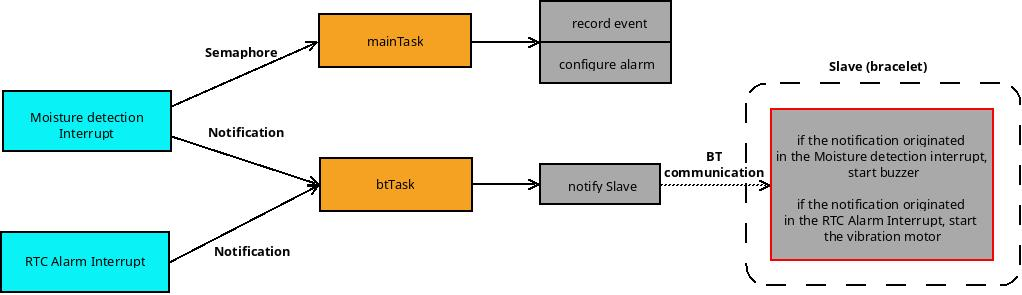
\includegraphics[width=\textwidth]{extInt.jpg}
         \caption{Moisture detection}
        \end{figure}
        
        It also configures the RTC module's TAR register (alarm) of the K64F for the following night for the time 15 minutes before the recorded event time using the {\bfseries configureAlarm()} function (listing ~\ref{lst:confAlarm}). The delay in this project is however, for the purpose of demonstration and development, set to 20 seconds only. 
        \begin{lstlisting}[label={lst:mdSemaphore}, caption=Moisture Detection Semaphore]
        if(xSemaphoreTake(moistureDetectionSemphr, 0))
        {
            PRINTF("\n\r\033[34mMoisture detected\033[0m\n\r");
            // flash an LED to indicate moisture detection
            for(int i = 0; i < 6; i++) {
                GPIO_PortToggle(BOARD_MD_LED_GPIO, 1 << BOARD_MD_LED_PIN);
                vTaskDelay(pdMS_TO_TICKS(150));
            }

            // store the event time in a struct array
            events[eventCount].eventTime = getSystemTime(RTC_1_PERIPHERAL, &RTC_1_dateTimeStruct);
            events[eventCount].eventDate = getSystemDate(RTC_1_PERIPHERAL, &RTC_1_dateTimeStruct);
            events[eventCount].wasAcknowledged = "no";

            // convert given structure to a single string and add it to a string array
            recordsAsStrings[eventCount] = convertRecordToString(events[eventCount]);

            eventCount++;

            // struct array set to 10 events only, this is a precaution
            if(eventCount > 9)
                eventCount = 9;

            configureAlarm(20);
            displayAlarmTime(RTC_1_PERIPHERAL, &RTC_1_dateTimeStruct);
		}	 
        \end{lstlisting}
        This interrupt also notifies the {\bfseries btTask} that an event occured and the btTask then transmits a notification to the Slave device to trigger a buzzer.
        
        The code below, shows the aforementioned {\bfseries recordsAsStrings()} function that converts the structure holding the time, date and acknowledgement status into a string and the {\bfseries configureAlarm()} function that configures the TAR register of the K64F. When the values of the RTC\_TSR register (time seconds register) and the RTC\_TAR register (time alarm register) match, the RTC module triggers an {\bfseries alarm interrupt} that notifies the {\bfseries btTask} to notify the {\bfseries Slave module} that in turn switches on the vibration motor.
        \begin{lstlisting}[label={lst:crtString}, caption=convertRecordToString()]
        char* convertRecordToString(struct eventData_t event)
        {
            // alocate memory for a string
            char* recordAsStrings = (char*) malloc(sizeof(char) * 21);

            strcpy(recordAsStrings, event.eventDate);
            strcat(recordAsStrings, SPACER);
            strcat(recordAsStrings, event.eventTime);
            strcat(recordAsStrings, SPACER);
            strcat(recordAsStrings, event.wasAcknowledged);

            return recordAsStrings;
        }
        \end{lstlisting}
        
        \begin{lstlisting}[label={lst:confAlarm}, caption=configureAlarm()]
        void configureAlarm(uint32_t secIncrement)
        {
            // configure alarm
            uint32_t currSec = 0;
            currSec = RTC->TSR;
            currSec += secIncrement;
            RTC->TAR = currSec;
        }
        \end{lstlisting}
        
        \subsubsection*{Time configuration}\label{section:timeConfig}
        \begin{figure}
         \centering
         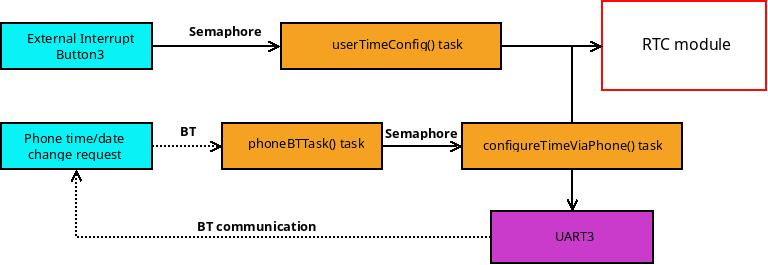
\includegraphics[width=\textwidth]{extInt_and_phone.jpg}
         \caption{Time configuration}
        \end{figure}

        In order to allow the user to configure time and date on the system I have enabled an external interrupt on Button3 of the K64F Master device. The configuration was initially performed using the terminal but the functionality got extended and can now be also performed using a mobile phone. When the external interrupt occurs a semaphore is given to the mainTask which creates a {\bfseries userTimeConfig} task (listing ~\ref{lst:userTimeConfig}). This task has higher priority than the main task so it takes over and displays appropriate information in the terminal window. The user can input time and date in specified format and if successful the new time and date is saved. The functionality is similar when the time and date change is requested via the phone, with the intermediary step of bluetooth communication. Instead of {\bfseries userTimeConfig} task a {\bfseries configureTimeViaPhone} task is created (listing ~\ref{lst:configureTimeViaPhone}).
        
        \begin{lstlisting}[label={lst:userTimeConfig}, caption=userTimeConfig() task]
        void userTimeConfig(void* pvParameters)
        {
            char stringDate[11] = "";
            char stringTime[6] = "";
            char stringTimeDate[17] = "";

            uint16_t newYear = 1970;
            uint8_t newMonth = 1, newDay = 1, newHour = 1, newMinute =1;

            for(;;)
            {
                RTC_StopTimer(RTC);

                PRINTF("\n\rEnter new date [min val 1970-01-01] in format YYYY-MM-DD: ");
                SCANF("%s", stringDate);

                // get date from the user input
                struct userDate_t newDate = getDate(stringDate);

                PRINTF("\n\rNew date: %s", stringDate);
                newYear = newDate.year;
                newMonth = newDate.month;
                newDay = newDate.day;

                while((newYear < 1970 || newYear > 2099) ||
                        (newMonth < 1 || newMonth > 12) ||
                        (newDay   < 1 || newDay > 31))
                {
                    PRINTF("\n\r*****  Invalid date [min val 1970-01-01] *****\n\r"
                            "Enter new date in format YYYY-MM-DD: ");
                    SCANF("%s", stringDate);

                    newDate = getDate(stringDate);

                    newYear = newDate.year;
                    newMonth = newDate.month;
                    newDay = newDate.day;
                }

                PRINTF("\n\rEnter new time in format HH-MM: ");
                SCANF("%s", stringTime);

                struct userTime_t newTime = getTime(stringTime);

                newHour = newTime.hour;
                newMinute = newTime.minute;

                while((newHour < 0 || newHour > 23) || (newMinute < 0 || newMinute > 59))
                {
                    PRINTF("\n\rInvalid time value, try again: ");
                    SCANF("%s", stringTime);

                    newTime = getTime(stringTime);

                    newHour = newTime.hour;
                    newMinute = newTime.minute;
                }

                RTC_1_dateTimeStruct.year = newYear;
                RTC_1_dateTimeStruct.month = newMonth;
                RTC_1_dateTimeStruct.day = newDay;
                RTC_1_dateTimeStruct.hour = newHour;
                RTC_1_dateTimeStruct.minute = newMinute;

                RTC_SetDatetime(RTC, &RTC_1_dateTimeStruct);
                memset(stringTimeDate, 0, sizeof(stringTimeDate));
                #ifdef SHOW_MESSAGES
                PRINTF("\n\rYear: %d", RTC_1_dateTimeStruct.year);
                PRINTF("\n\rMonth: %d", RTC_1_dateTimeStruct.month);
                PRINTF("\n\rDay: %d", RTC_1_dateTimeStruct.day);
                PRINTF("\n\rHour: %d", RTC_1_dateTimeStruct.hour);
                PRINTF("\n\rMinute: %d\n\n\r", RTC_1_dateTimeStruct.minute);
                #endif
                RTC_StartTimer(RTC);
                vTaskDelete(NULL);
            } // end of for(;;)
        } // end of userTimeConfig task
        \end{lstlisting}
        
        \begin{lstlisting}[label={lst:configureTimeViaPhone}, caption=configureTimeViaPhone() task]
         void configureTimeViaPhone(void* pvParameters)
        {

            uint8_t receivedDateTime[17];
            char* enterValDateTime = "Please enter valid dateTime in [YYYYMMDD-HHMM] format";

            PRINTF("\n\r\033[33mIn configure time via phone\033[0m");

            for(;;) {
                UART_WriteBlocking(UART3, (uint8_t*)enterValDateTime, strlen(enterValDateTime) + 1 );

                switch(UART_ReadBlocking(UART3, receivedDateTime, 17)) {
                    case kStatus_Success : 	PRINTF("\n\rReceived: %s", receivedDateTime);
                        configureAndDisplayNewTime(receivedDateTime);
                        break;
                    case kStatus_UART_RxHardwareOverrun : 	PRINTF("\n\rHardware Overrun"); 
                        break;
                    case kStatus_UART_NoiseError 		: 	PRINTF("\n\rNoise Error"); 
                        break;
                    case kStatus_UART_FramingError 		: 	PRINTF("\n\rFraming Error"); 
                        break;
                    case kStatus_UART_ParityError 		: 	PRINTF("\n\rParity Error"); 
                        break;
                    default								: 	PRINTF("\n\rUnknown Error"); 
                        break;
                }
                vTaskDelete(NULL);
            }
        }
        \end{lstlisting}
        The configureTimeViaPhone task uses {\bfseries configureAndDisplayNewTime() function} that in it's functionality resembles the terminal version. The main difference is that the information from this function is sent via Bluetooth through the UART3 peripheral to the phone (listing ~\ref{lst:btTimeConfig}). Please, see the relevant snippets below. 
        \begin{lstlisting}[label={lst:btTimeConfig}, caption=Time and date BT communication]
        char* systemDate = getSystemDate(RTC_1_PERIPHERAL, &RTC_1_dateTimeStruct);
        UART_WriteBlocking(UART3, (uint8_t*)"System date set to: ", strlen("System date set to: ") + 1);
        UART_WriteBlocking(UART3, (uint8_t*)systemDate, strlen(systemDate) + 1);
        \end{lstlisting}
        
        \subsubsection*{Phone BT task}
        As mentioned earlier, this task is one of the first once created in the main(). It is mainly responsible for receiving communication from the phone's Bluetooth and in few instances also returns data back to it. This task continously checks the status of {\bfseries Receive Data Register Full Flag}. If this flag is set, it proceeds to read data from the UART3 data register and evaluates them. A switch is used to specify the course of action the taks should take (listing ~\ref{lst:phoneBTTaskSwitch}). The received values have been defined in the {\bfseries bluetooth2.h} file for better readability of the code.\\
        
		\begin{itemize}[topsep=4pt,itemsep=1pt]
            \item DEV\_ALARM\_STOP - stops the ongoing alarm on the Slave device. It uses a FreeRTOS queue that transfers the received character through btTask to Dev2 (bracelet). This is because the phoneBTTask cannot directly communicate with the secondary device. This is responsibility of the {\bfseries btTask}. The queue forms a sort of bridge between these two.
            \item SYSTEM\_TIME\_REQUEST - requests system time from the RTC module and sends the value back to the phone  
            \item SYSTEM\_DATE\_REQUEST - requests system date from the RTC module and sends the value back to the phone 
            \item SYSTEM\_TIME\_CHANGE - system time and date configuration via mobile phone as discussed in section ~\ref{section:timeConfig} on the page \pageref{section:timeConfig}.   
            \item REQUEST\_RECORDS - requests recorded times and dates of incidents  
		\end{itemize}
		
		All the functions above are fairly self-explanatory however I would like to elaborate a bit on the REQUEST\_RECORDS item. As mentioned previously, every time an event occurs, current time and date is stored in a structure that then gets converted into a string and stored in a string array. To being able to receive data from this array I had to use a FreeRTOS queue to transfer this data from the mainTask, where it was stored, to the phoneBTTask first. When the mainTask receives the semaphore from the phoneBTTask, it puts the string array into this queue where it can be retrieved by the phoneBTTask for further processing. In this case this means sending the data to the phone via Bluetooth (UART3).
        
        \begin{lstlisting}[label={lst:phoneBTTaskSwitch}, caption=Phone request resolution]
        if(kUART_RxDataRegFullFlag & UART_GetStatusFlags(UART3)) {
            charReceived = UART_ReadByte(UART3);
            switch(charReceived) {
                case DEV2_ALARM_STOP: 		
                    xQueueSend(phoneBTReceiveQ, (void*)&charReceived,
                    pdMS_TO_TICKS(0)); 
                    break;
                case SYSTEM_TIME_REQUEST: 	
                    sendDataToPhone(getSystemTime(RTC_1_PERIPHERAL, &RTC_1_dateTimeStruct));
                    break;
                case SYSTEM_DATE_REQUEST: 	
                    sendDataToPhone(getSystemDate(RTC_1_PERIPHERAL, &RTC_1_dateTimeStruct));
                    break;
                case SYSTEM_TIME_CHANGE:	
                    PRINTF("System time change\n\r");
                    charReceived = '\0';
                    xSemaphoreGive(configureTimeViaPhoneSemphr);
                    break;
                case REQUEST_RECORDS:		
                    PRINTF("\n\r\033[33mRequesting records...\033[0m\n\r");
                    xSemaphoreGive(recordsRequestSemphr);

                    if(xQueueReceive(recordsForThePhoneQ, &recordsForPhoneBuffer, pdMS_TO_TICKS(200)))
                    {
                        PRINTF("\033[32mData received!!!\033[0m\n\r");
                        PRINTF("\n\r\033[32mSending data to Phone!!!\033[0m\n\r");

                        int i = 0;
                        while(recordsForPhoneBuffer[i] != 0x0)
                        {
                            sendDataToPhone(recordsForPhoneBuffer[i]);
                            busyDelay(20000);
                            i++;
                        }
                        PRINTF("\n\r\033[32mData send!!!\033[0m\n\r");
                    }
                    break;
                default:					
                    PRINTF("Invalid request\n\r"); charReceived = '\0'; break;
            } 
            charReceived = '\0';
            UART_ClearStatusFlags(UART3,  kUART_RxDataRegFullFlag);
        } 
        \end{lstlisting}
        
    This would conclude the main functionality of the Master device. There is a lot more code in the project that can be viewed in the repository by following the link provided just below this section's title. I would like to mention the {\bfseries helper\_functions.c} file where I've put some of the helping functions in an attempt to keep things tidy. I have tried to divide the code logically into separate .c and .h files as well. I have also used Doxygen to generate documentation for the various elements and this can be viewed by navigating into <repository\_path>/Docs/api\_docs/html/index.html Trying to view this on GitHub directly isn't possible. Navigating to this file results in the source code for this Doxygen documentation. 
    
   \subsection{K64F Slave code development}
   \href{https://github.com/zedd-1983/project_dev2/tree/Bluetooth}{K64F Slave (Bracelet) Device code repository}\\
   
   \begin{figure}[h]
    \centering
    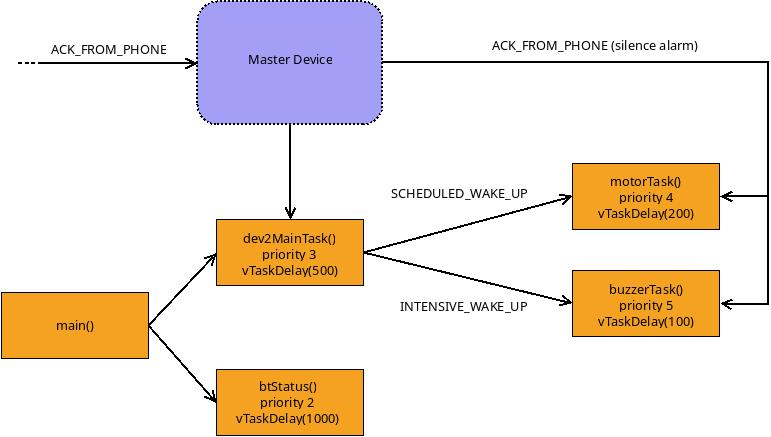
\includegraphics[width=\textwidth]{dev2_functionality.jpg}
    \caption{Slave functionality}
    \label{fig:dev2Func}
   \end{figure}
   The functionality of the Slave device is not as complicated as the functionality of the Master. It's responsibility lies in waking up the sleeping person. It does so by activating either a buzzer or a vibration motor, based on the notification it receives from the Master device via Bluetooth. 
   Setting up this device wasn't as complex and as I already had some experience from setting up the Master and it's Bluetooth module, this proved quite simple. I have used the MCUXpresso Config Tool (fig. ~\ref{fig:flexTimerConfig}) to configure the {\bfseries Flex Timer Module} of the K64F so I could generate a square wave on the pin where the buzzer is connected. This allowed me to specify the output frequency of this square wave thus changing the pitch of the emitted sound. It is possible to do this configuration programmatically, however using the Configuration tool is less error prone and easier.
   
    \begin{figure}[h]
        \centering
        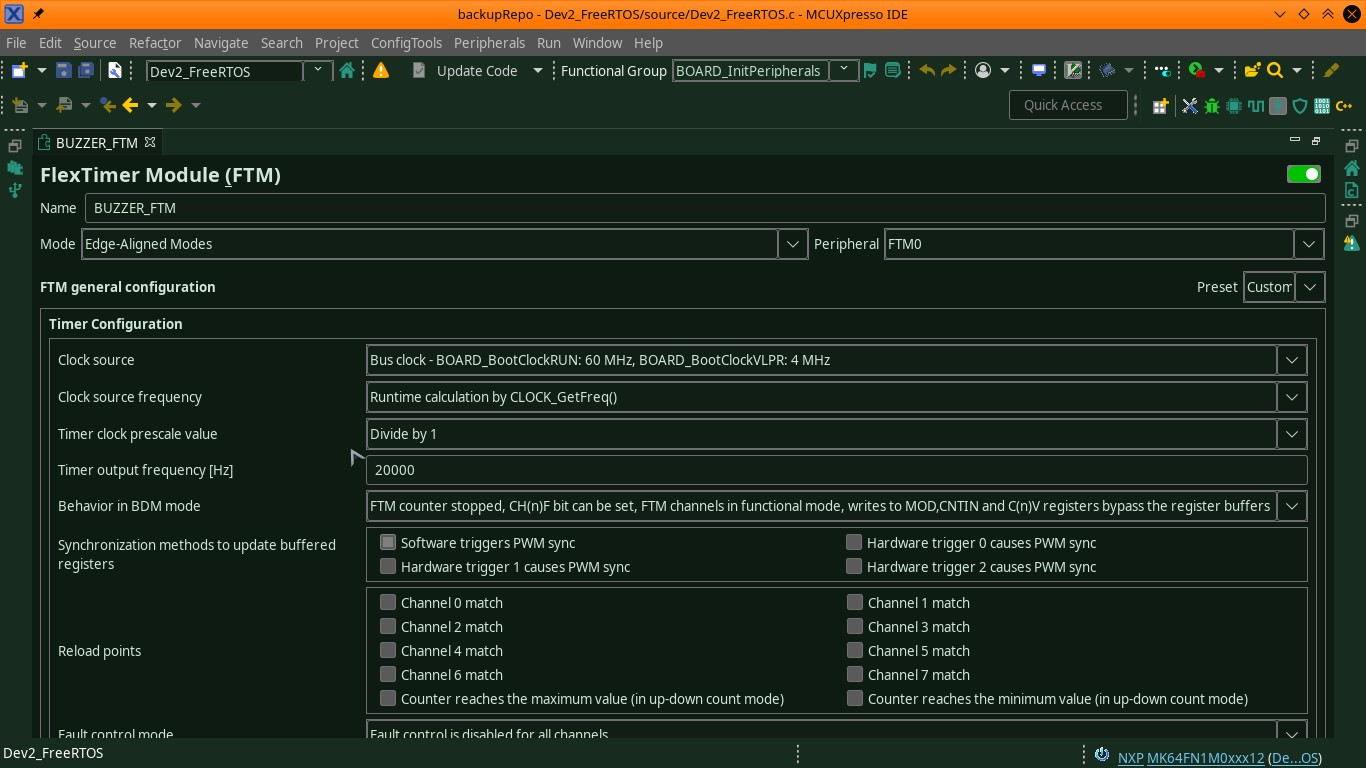
\includegraphics[width=\textwidth]{FlexTimer_config.jpeg}
        \caption{MCUXpresson Configuration Tool}
        \label{fig:flexTimerConfig}
    \end{figure}
    
    As the complexity of the code running on the Slave device isn't too complex, I have left everything in just one file. 
    
    \subsubsection*{main()}
    The main function is responsible for creating two FreeRTOS tasks and to start the scheduler. The two tasks are {\bfseries dev2MainTask} and {\bfseries btStatus} task.
    
    \subsubsection*{btStatus() task}
    The sole responsibility of this task, is to listen for the input on the PTC16 to go HIGH. This pin is connected to the status pin of the HC-05 module and if HIGH, indicates that the connection with another module has been established. To indicate this on the K64F, a BLUE LED is turned on to steady light. Otherwise it flashes. 
    
    \begin{lstlisting}[label={lst:btStatus}, caption=btStatus() task]
    void btStatusTask(void* pvParameters)
    {
        for(;;)
        {
            if(GPIO_PinRead(BOARD_BT_STATE_GPIO, BOARD_BT_STATE_PIN) == 1)
                GPIO_PinWrite(BOARD_BLUE_LED_GPIO, BOARD_BLUE_LED_PIN, 0);
            else
                GPIO_PortToggle(BOARD_BLUE_LED_GPIO, 
                    1 << BOARD_BLUE_LED_PIN);
            vTaskDelay(pdMS_TO_TICKS(500));
        }
    }
    \end{lstlisting}
    
    \subsubsection*{dev2MainTask() task}
    This task listens for the messages comming in via UART4 (Bluetooth) in the same fashion as the {\bfseries phoneBTTask()} on the Master device. If there are some messages, it evaluates them and decides what to do next. There are currently three types of messages that can be dealt with.\\
    
    \begin{itemize}[topsep=4pt, itemsep=1pt]
     \item SCHEDULED\_WAKE\_UP - this is the main event. This is received as the action of the Master device based on the recording of the incidents and starts the vibration motor task.
     \item INTENSIVE\_WAKE\_UP - this is triggered, when an event occurs (the child wets the bed), and it starts the buzzer task
     \item ACK\_FROM\_PHONE - this is a ongoing alarm silence measure. It is received, when the user wants to silence the alarm by phone
    \end{itemize}
    
    \begin{lstlisting}[label={lst:dev2MainTask}, caption=dev2MainTask() task]
    void dev2MainTask(void* pvParameters)
    {
    #ifdef DEBUG_MSG
        PRINTF("\n\rMain Task\n\r");
    #endif
        for(;;)
        {
            if(kUART_RxDataRegFullFlag & UART_GetStatusFlags(UART4)) {
                uint8_t charReceived = UART_ReadByte(UART4);
                if(charReceived == SCHEDULED_WAKE_UP) {
                    charReceived = 0;
                    GPIO_PortToggle(BOARD_RED_LED_GPIO, 1 << BOARD_RED_LED_PIN);
                    PRINTF("\n\rAlarm");
                    if(xTaskCreate(motorTask, "Motor task", configMINIMAL_STACK_SIZE + 100, NULL, 4, &motorTaskHandle) == pdFALSE)
                    {
                        PRINTF("\n\rMotor Task creation failed");
                    }
                }
                else if(charReceived == INTENSIVE_WAKE_UP) {
                    charReceived = 0;
                    PRINTF("\n\rBuzzer");
                    if(xTaskCreate(buzzerTask, "Buzzer task", configMINIMAL_STACK_SIZE + 100, NULL, 5, &buzzerTaskHandle) == pdFALSE)
                    {
                        PRINTF("\n\rBuzzer Task creation failed");
                    }
                }
                else if(charReceived == ACK_FROM_PHONE)
                {
                    charReceived = 0;
                    PRINTF("\n\rACKNOWLEDGED from PHONE");
                    xSemaphoreGive(ackSemphr);
                }
            }
            vTaskDelay(pdMS_TO_TICKS(1000));
        }
    }
    \end{lstlisting}
    
    \subsubsection*{motorTask()}
    This task simply turns a pin HIGH, when it is started, thus starting a vibration motor through the circuit (fig. ~\ref{fig:vibMotorConnDiag}) discussed on the page \pageref{fig:vibMotorConnDiag}. This task will delete itself when it receives acknowledgement semaphore from the dev2MainTask (based on the received message from the Bluetooth).

    \begin{lstlisting}[label={lst:motorTask}, caption=motorTask() task]
    void motorTask(void* pvParameters)
    {
        PRINTF("\n\rMotor (scheduled wake-up) task created");
        for(;;)
        {
            GPIO_PortToggle(BOARD_RED_LED_GPIO, 1 << BOARD_RED_LED_PIN);
            vTaskDelay(pdMS_TO_TICKS(200));

            if(xSemaphoreTake(ackSemphr, 0) == pdTRUE)
            {
                GPIO_PinWrite(BOARD_RED_LED_GPIO, BOARD_RED_LED_PIN, 1);
                PRINTF("\n\rMotor task deleted");
                vTaskDelete(NULL);
            }
        }
    }
    \end{lstlisting}
    
    \subsubsection*{buzzerTask()}
    This task starts the passive buzzer connected to PTC1. This pin is configured to produce a square wave through the Flex Timer Module rather than creating the square wave by way of toggling the pin manually. It is silenced when it receives the acknowledgement semaphore from the dev2MainTask.
    \begin{lstlisting}[label={lst:buzzerTask}, caption=buzzerTask()]
     void buzzerTask(void* pvParameters)
    {
        PRINTF("\n\rBuzzer (intensive wake-up) task created");
        FTM_StartTimer(BUZZER_FTM_PERIPHERAL, BUZZER_FTM_CLOCK_SOURCE);

        
        for(;;)
        {
            vTaskDelay(pdMS_TO_TICKS(1000));

            if(xSemaphoreTake(ackSemphr, 0) == pdTRUE)
            {
                FTM_StopTimer(BUZZER_FTM_PERIPHERAL);
                PRINTF("\n\rBuzzer task deleted");
                vTaskDelete(NULL);
            }
            vTaskDelay(pdMS_TO_TICKS(100));
        }
    }
    \end{lstlisting}

    \subsection{Android application code development}
    \href{https://github.com/zedd-1983/Easysleep_app/tree/bt_connection_3}{Android code repository}\\
    
    The aim of developing the phone application for the Easysleep project, was to allow the user to control the two embedded devices remotely. Before deciding to develop this application, I was using a third-party software downloaded from Google Play Store to my phone to send and receive data via Bluetooth. This allowed me to test the Bluetooth communication functionality of the embedded devices before attempting to wrap it into a nicer user friendly interface.
    
                
    \subsubsection{User Interface Development}
    Graphical User Interface\\
    
    \begin{wrapfigure}{R}{0.4\textwidth}
        \centering
        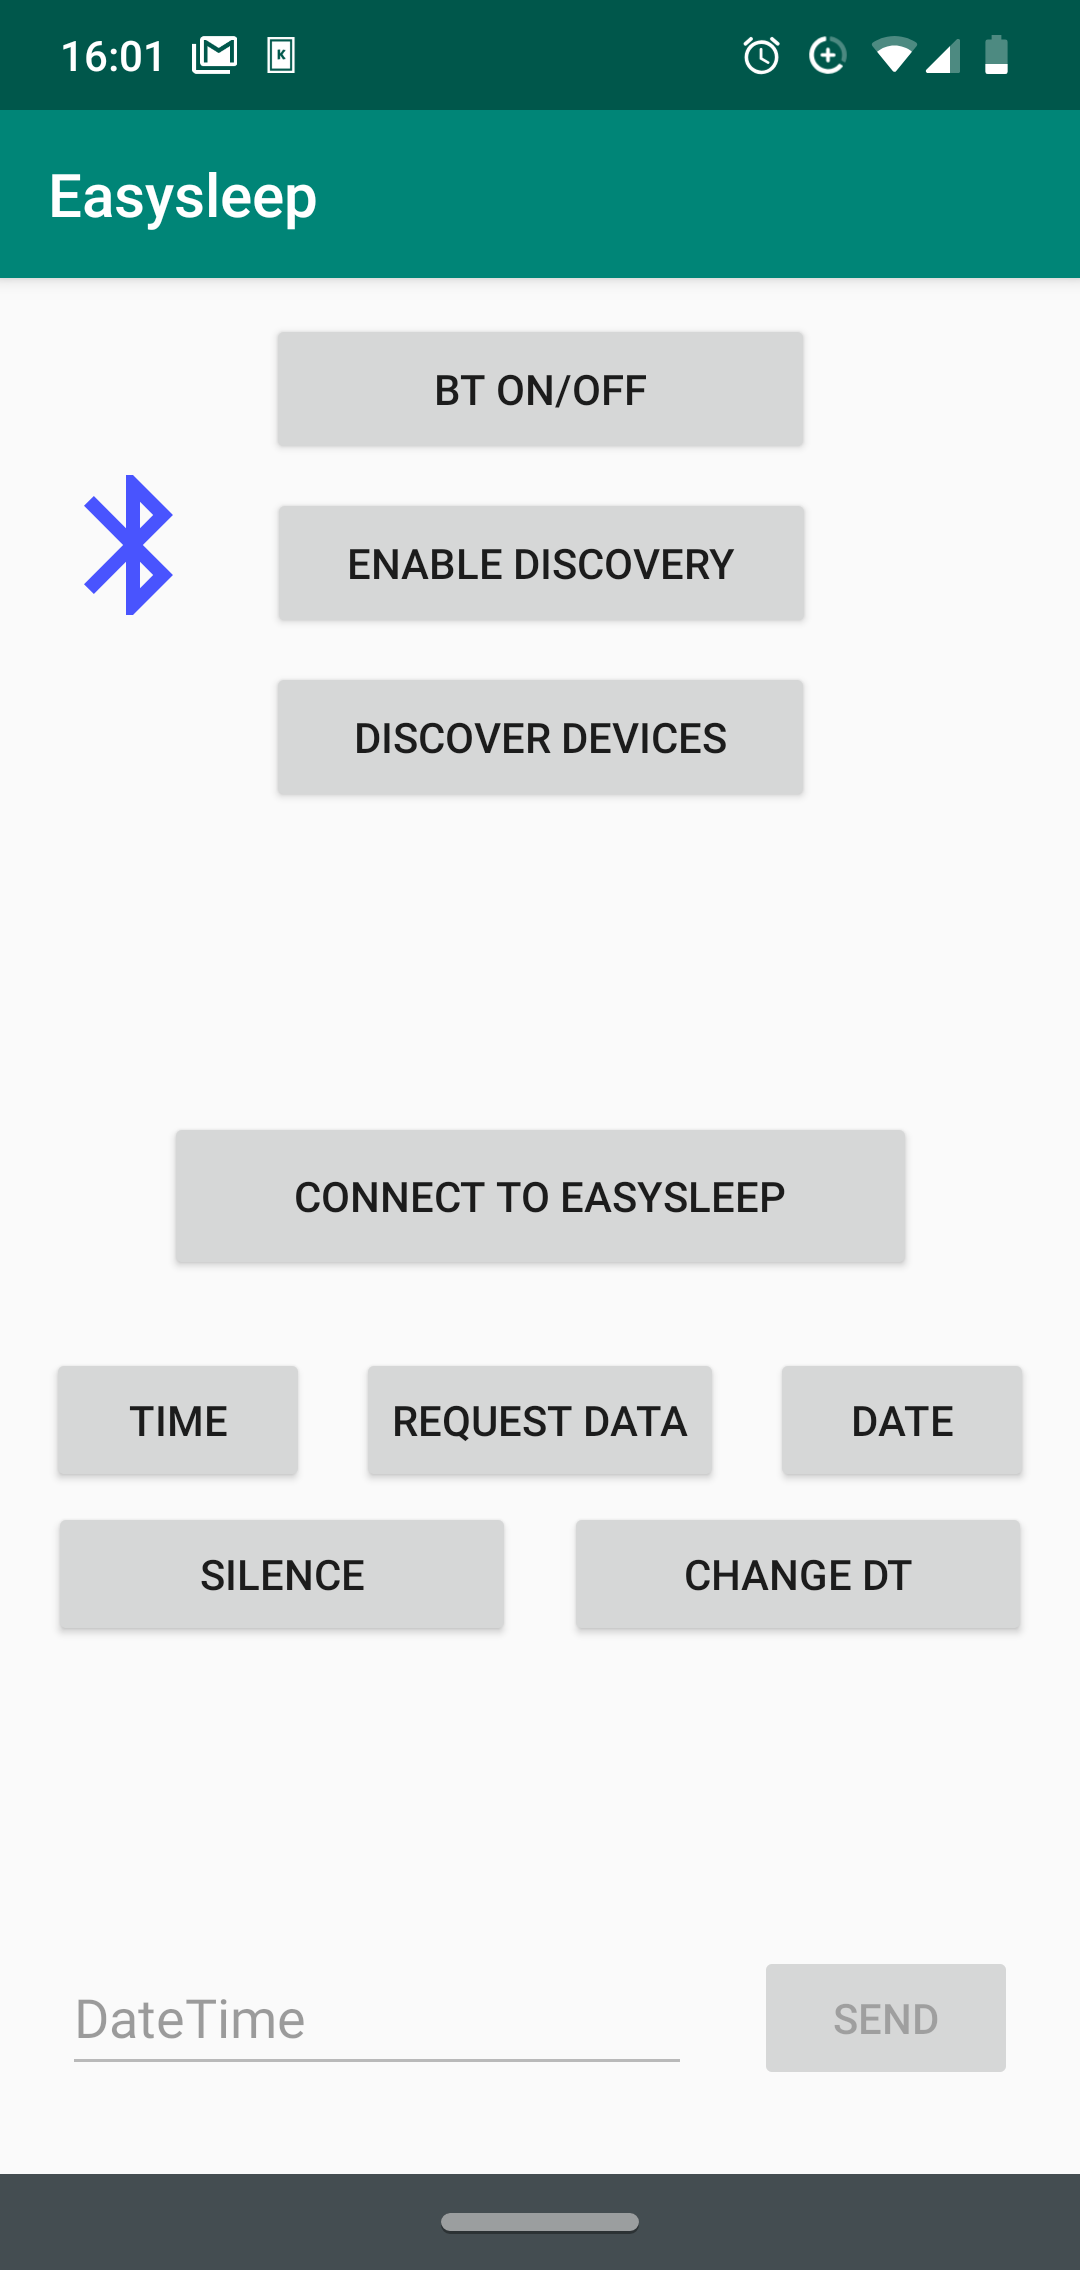
\includegraphics[scale=0.1]{easysleep_app.png}
        \caption[Easysleep Application]{Easysleep}
    \end{wrapfigure}
    I have gone through few versions of UI of this application during the course of the development. Initially, the UI consisted of only four buttons that would allow me to toggle the Bluetooth on the phone, display a list of known devices or make the phone visible to others. However, as the functionality grew and changed, so did the user interface.\\
    
    In the top section of the screen are buttons that interract with the Bluetooth module of the phone, while in the bottom section are buttons that the user can use to communicate with the Easysleep Master device as well as a text field to display results of messages from it. The functionality of the buttons doesn't need further explanation as the text of the buttons is quite self-explanatory.\\
    
    I have used the Layout Designer which is part of the Android Studio, to create the layout of various elements of the UI. I've linked these elements through their {\bfseries id} with corresponding classes in the onCreate() method. This allowed me to assign action listeners to them and specify the functionality if any of the buttons are clicked.

    
    
   
   \subsubsection{Bluetooth Communication}
   BT\\
   \subsubsection{Database Development}
   ???\\
               
   The development of this application was challenging and I had to follow a number of tutorials online in order to establish the Bluetooth communication. I have decided that for the purpose of this document I will divide the development process described into three subsections:  
               
   \begin{itemize}
    \item User Interface Development
    \item Bluetooth Communication
    \item Database Development
   \end{itemize}
    
    \section{References}
    \newpage

    \section{Bibliography}
    \newpage

    \section{Figures}
    \listoffigures
    \newpage

    \section{Code listings}
    \lstlistoflistings
    \newpage

\end{document}
